% Created 2014-06-27 Fri 18:47
\documentclass{article}
\usepackage[utf8]{inputenc}
\usepackage[T1]{fontenc}
\usepackage{fixltx2e}
\usepackage{graphicx}
\usepackage{longtable}
\usepackage{float}
\usepackage{wrapfig}
\usepackage{soul}
\usepackage{textcomp}
\usepackage{marvosym}
\usepackage{wasysym}
\usepackage{latexsym}
\usepackage{amssymb}
\usepackage{hyperref}
\tolerance=1000
\usepackage[margin=1in]{geometry}
\usepackage[round]{natbib}
\usepackage[nonumberlist]{glossaries}
\usepackage{enumitem}
\setlist{nolistsep}
\usepackage{graphicx}
\newglossaryentry{pc}{name={PC}, description={Pitch Class}}
\newglossaryentry{pcset}{name={PC-Set}, description={Pitch Class Set}}
\newglossaryentry{sc}{name={SC}, description={Set Class}}
\newglossaryentry{nc}{name={nC}, description={Cardinality Class}}
\newglossaryentry{hashnc}{name={\#nC}, description={Size of nC}}
\newglossaryentry{ic}{name={IC}, description={Interval Class}}
\newglossaryentry{tnx}{name={Tn(X)}, description={Transposition}}
\newglossaryentry{ix}{name={I(X)}, description={Inversion}}
\newglossaryentry{tntype}{name={Tn-Type}, description={Transpositional SC-type}}
\newglossaryentry{itype}{name={I-Type}, description={Inversional SC-Type}}
\newglossaryentry{tnitype}{name={TnI-Type}, description={Transpositional/Inversional SC-Type}}
\newglossaryentry{primeform}{name={Prime Form}, description={PC-set representing all members of an SC}}
\newglossaryentry{icv}{name={ICV}, description={Interval-class Vector}}
\newglossaryentry{ncv}{name={nCV}, description={n-class subset vector}}
\newglossaryentry{ncpv}{name={nC\%V}, description={n-class subset percentage vector}}
\newglossaryentry{nsatv}{name={nSATV}, description={n-class subset saturation vector}}
\newglossaryentry{dv}{name={DV}, description={Difference Vector}}
\newglossaryentry{hashx}{name={\#X}, description={Set cardinality}}
\newglossaryentry{hashncv}{name={\#nCV}, description={Vector cardinality}}
\newglossaryentry{trivialform}{name={Trivial Form}, description={SCs 1-1, 11-1 and 12-1}}
\makeglossaries
\providecommand{\alert}[1]{\textbf{#1}}

\title{Evaluation of Pitch-Class Set Similarity Measures for Tonal Analysis (Draft)}
\author{Nicholas Harley - Masters Thesis UPF}
\date{\today}
\hypersetup{
  pdfkeywords={},
  pdfsubject={},
  pdfcreator={Emacs Org-mode version 7.9.3f}}

\begin{document}

\maketitle

\setcounter{tocdepth}{3}
\tableofcontents
\vspace*{1cm}


\clearpage
\glsaddall
\printglossary[title=PC-Set Theory Glossary]
\%makeindex -s doc.ist -o doc.gls doc.glo
\clearpage
\section{Introduction}
\label{sec-1}

The objectives of the present work are principally concerned with
descriptive modelling of tonality using PC-set theory. In particular,
the analytical potential of set-class similarity measures will be
assessed and evaluated through comparison with similar work. The
tentative goal, therefore, is to present this approach in such a way
as to make it relevant to the wider community of music researchers,
such as those in MIR.

Chapters \ref{sec-2}-\ref{sec-5} comprise a literature
review containing background information and some basic
theory. Chapter \ref{sec-2} addresses the challenges and problems
involved in descriptive modelling of tonality as a means of
justification for the proposed approach. Chapter \ref{sec-3} introduces the basic concepts of PC-set theory including
set-class similarity measures. Chapter \ref{sec-4}
gives a basic description of MDS techniques and how they can play a
role in set-class analysis. Chapter \ref{sec-5}
contains a review of the relevant tonal models that exist so as to
give context work that follows.
\section{Tonality}
\label{sec-2}
\subsection{Defining Tonality}
\label{sec-2-1}
\subsubsection{General Definition}
\label{sec-2-1-1}

Tonality is a notoriously complex musical phenomenon and numerous
definitions have been proposed from a variety of viewpoints. Perhaps
the most general definition is that provided by \citet{Hyer2013}:
``\ldots{} refers to the systematic arrangements of pitch phenomena and
relations between them.'' Explanations of tonality have been provided
through many different disciplines (acoustics, music theory,
linguistics, cognitive psychology) and a detailed discussion of these
areas is certainly beyond the scope of this work. However, it is
generally agreed that tonality is an abstract cultural and cognitive
construct that can have many different physical representations.
\subsubsection{Babbitt's Domains}
\label{sec-2-1-2}

\citet{Babbitt1965} proposed three domains to categorise different
types of representation of music: acoustic (physical), auditory
(perceived), graphemic (notated). Western music theory provides a
lexicon for describing abstract tonal objects with terms such as note,
chord and key. These objects have a hierarchical relationship and the
meaning of these labels is highly dependent on musical context and the
scale of observation. Musicological descriptions, which constitute the
majority of reasoning about tonaility, reside mainly in the Babbitt's
graphemic domain, although arguably they reflect some aspects of the
other two. Each domain, whilst connected to every other, provides only
a projection of the musical whole and examination of tonality from
just one will most likley result in an incomplete picture. However,
these three domains provide a convenient framework for the discussion
that follows.
\subsection{Modelling Tonality}
\label{sec-2-2}

The challenge of mathematically modelling aspects of tonality has been
approached in numerous ways and from different domains. In the
graphemic domain, musicologists and composers have proposed
theoretical models, attempting to rethink tonal theory from a
mathematical perspective. These models employ different branches of
mathematics such as geometry \citep{Tymoczko2012} or group theory
\citep{Ring2011} to describe harmonic structure. From the auditory
domain, cognitive psychologists have built models of tonal induction
based on perceptual ratings of tonal stimuli \citep{Krumhansl1990}.
\subsubsection{Tonality as Context}
\label{sec-2-2-1}

Many models approach the concept of tonality as a context, within
which the relations and hierarchies of tonal phenomena can be
understood. A sense of tonality can be induced when musical stimuli
resemble some a priori contextual category. For western music of the
major-minor period, key signatures comprise a collection of categories
that give context to the tonal components of
music. \citet{Martorell2013} identifies three important aspects of
tonality as context: dimensionality (the relatedness or ``closeness'' of
categories), ambiguity (reference to two or more categories
simultaneously) and timing (the dynamics of tonal context). He
highlights the importance of a models capability to describe these
aspects. 
\subsubsection{Tonality in MIR}
\label{sec-2-2-2}

The MIR community is primarily concerned with the extraction of tonal
descriptors from audio signals such as chord and key estimates. Most
systems use chroma features as a preliminary step, obtained by mapping
STFT or CQ transform energies to chroma bins. Template matching is
used to compare the chroma vectors to a tonal model (contextual
category) using some distance measure. A commonly used tonal model for
key estimation are the KK-profiles \citep{Krumhansl1990} (\ref{sec-5-3}) (e.g. in \citealt{Gomez2006}). Distance measures such as
inner product (e.g. in \citealt{Gomez2006}) and fuzzy distance
(e.g. in \citealt{Purwins2000}) are used to compare
vectors. Statistical methods, such as HMMs, have been used for chord
and key tracking \citep{Chai2005}. Of addition interest in the field
is the concept of musical similarity (for music recommendation,
structure analysis, cover detection etc.). \citet{Foote2000} computed
self-similarity matrices for visualisation of structure by correlating
the MFCC feature vector time-series. \citet{Gomez2006} proposed the
application of this method to tonal feature vectors.
\subsubsection{Similarity}
\label{sec-2-2-3}

The importance of defining the similarity or closeness between musical
phenomena, be it theoretical, physical or perceptual, is central to
almost every model of tonality and often leads to a geometric
configuration of tonal objects. The concepts of similarity and
distance is discussed further in Chapter \ref{sec-5}
where a review of spatial models of tonality is given.
\subsection{The Semantic Gap}
\label{sec-2-3}
\subsubsection{Acoustic Domain}
\label{sec-2-3-1}

\citet{Wiggins2009} discusses, what is referred to in MIR as, the
``Semantic Gap'': the inability of systems to achieve success rates
beyond a conspicuous boundary. He examines the fundamental
methodological groundings of MIR in terms of Babbitts three domains,
discussing the limits of each representation and regarding the
discarnate nature of music. He concludes that the audio signal
(acoustic domain) simply cannot contain all of the information that
systems seek to retrieve. He points towards the the auditory domain as
the chief residence of music information and urges for in not to be
overlooked in MIR and wider music research.
\subsubsection{Graphemic Domain}
\label{sec-2-3-2}

Furthermore, Wiggins criticises the purely graphemic approach and the
tendency of music research to presuppose musicological
axioms. \citet{Wiggins2012} argues that music (tonal) theory is,
rather than a theory in the scientific sense, a highly developed folk
psychology (internal human theory for explaining common
behaviour). Thus, the rules of music theory are not like scientific
laws but rather abstract descriptions of a specific musical
behaviour. This idea challenges the validity of formalising such rules
in mathematics and prompts the question, ``What is actually being
modelled?'' He concludes that to apply mathematical models to musical
output alone (scales or chords) without consideration of the musical
mind is a scientific failure.
\subsubsection{Problems}
\label{sec-2-3-3}

The two assertions of Wiggins sit contrary to a number of the aspects
of the tonal models discussed in \ref{sec-2-2}. Firstly, the
major-minor paradigm, upon which so many approaches are based, whilst
certainly possessing cognitive significance, is still a musicological
concept and therefore a misleading basis for both mathematical and
cognitive approaches. A second problem is that of the numerical
methods used by some MIR systems, in particular, distance measures. As
will be discussed in Chapter \ref{sec-5}, similarity
(and by extension distance) is a central part of the auditory
domain. MIR systems often uses distance measures from mathematics such
as Mahalanobis \citep{Tzanetakis1999} or Cosine \citep{Foote2000} with
little consideration of their perceptual or musical significance.
\subsection{Systematicity}
\label{sec-2-4}
\subsubsection{The Musical Surface}
\label{sec-2-4-1}

Having cautioned against a purely musicological approach,
\citet[pp. 481]{Wiggins2009} proposes a compromise: to adopt a
bottom-up approach to music theory, exploring the concepts through
systematic mid-level representations. He states that ``methods
starting at, for example, the musical surface of notes is a useful way
of proceeding'' The concept of musical surface is illustrated by
\citet[pp. 159]{Huovinen2007} with a metaphor: ``\ldots{}to approach a
musical landscape not by drawing a map, which necessarily confines
itself to a limited set of structurally important features, but by
presenting a bird’s-eye view of the musical surface – an aerial
photograph, as it were, which details the position of every pitched
component.''
\subsubsection{Systematic Description}
\label{sec-2-4-2}

\citet{Martorell2013} also advocates this mid-level approach,
observing that surface description influences analyitcal observation
and that, for an unbiased view, the researcher must be provided with
the adequate raw materials with which to make more in-depth
observation. Such a systematic, descriptive model would be
fundamentally independent of high level concepts such as chords and
key but, at the same time, capable of capturing
them. \citet{Martorell2013} also discusses the importance of
systematicity in terms of dimensionality, ambiguity and timing. He
finds that models based on the major-minor paradigm are incapable of
adequately describing tonal ambiguity even in some Western music
\citep[chap. 3]{Martorell2013}.

With a systematic description of the musical surface, theories and
models from different domains can be gathered and evaluated together in
the same analytical arena, thus helping to bridge the gap between
traditional musicology, cognitive psychology and MIR.
\section{Pitch-Class Set Theory}
\label{sec-3}

One such method available for systematic description of the musical
surface is Pitch class set theory. PC-set theory is a system for
analysing the pitch content of music. It uses class equivalence
relations to reduce the amount of data required to describe any
collection of pitches. This chapter will outline the basic principles.
\subsection{Pitch Class}
\label{sec-3-1}

Pitch-class set theory uses octave equivalence. In Western equal
temperament (TET), a pitch-class (PC) is an integer representing the
residue class modulo 12 of a pitch \citep(Babbit1955) and indicates
the position of a note within the octave. A PC-set is a collection of
PCs ignoring any repetitions and the order in which they
occur. PC-sets are notated as follows \{0,1,2,3,4\} with PCs ordered
from lowest to highest as a convention (Example 1). The cardinality of
a set, denoted \#S, is the number of PCs it contains (Example 2). There
are 4096 (2$^{\mathrm{12}}$) unique PC-sets with which any segment of music can be
represented.

\begin{table}[htb]
\caption{Notes and corresponding pitch-classes} 
\begin{center}
\begin{tabular}{lrrrrrrrrrrrr}
 Note  &  C  &  C\#  &  D  &  D\#  &  E  &  F  &  F\#  &  G  &  G\#  &  A  &  A\#  &   B  \\
 PC    &  0  &    1  &  2  &    3  &  4  &  5  &    6  &  7  &    8  &  9  &   10  &  11  \\
\end{tabular}
\end{center}
\end{table}



\begin{center}
\begin{tabular}{llll}
 Example 1:  &  PC-set       &  Pitch-set  &  S = \{A4,C5,E5,A5\} (A minor)  \\
             &               &  PC-set     &  S = \{9,0,4,9\} = \{0,4,9\}    \\
 Example 2:  &  Cardinality  &             &  \#S = 3                        \\
\end{tabular}
\end{center}
\subsection{Set Classification}
\label{sec-3-2}

Defining equivalence classes of PC-sets further reduces the total
number of tonal objects. A set-class (SC) is a group of PC-sets
related by a transformation or group of transformations. The two types
of transformation commonly used are transposition and inversion. A
transposition, Tn(S), transposes the set, S, by the interval, n, (by
adding n to all PCs, Example 3). An inversion, I(S), inverts the set
S, replacing all PCs with their inverse (12-PC, Example 4). From these
two transformations it is possible to define three types of SC: Tn,
TnI and I.


\begin{center}
\begin{tabular}{lll}
 Example 3:  &  Transposition  &  S = \{0,4,9\}, T3(S) = \{3,7,0\} = \{0,3,7\}   \\
 Example 4:  &  Inversion      &  S = \{0,4,9\}, I(S) = \{11,7,2\} = \{2,7,11\}  \\
\end{tabular}
\end{center}



\begin{description}[style=multiline,leftmargin=2.5cm,font=\normalfont]
\item[Transpositional (Tn)] All PC-sets that can be transformed to each by transposition belong to the same class.There are 348 distinct Tn types.
\item[Inversional (I)] All PC-sets that can be transformed to each other by inversion belong to the same SC. There are 197 distinct I types.
\item[Transpositional/Inversional (TnI)] All PC-sets that can be transformed to each other by transposition, inversion or both belong to the same SC. There are 220 distinct TnI types.
\end{description}


\begin{center}
\begin{tabular}{ll}
 Transpositional (Tn):  &  All PC-sets that can be transformed to each  \\
                        &  by transposition belong to the same class.   \\
                        &  There are 351 distinct Tn types.             \\
 Inversional (I):       &  All PC-sets that can be transformed to each  \\
                        &  other by inversion belong to the same SC.    \\
                        &  There are 200 distinct I types.              \\
 Transpositional/       &  All PC-sets that can be transformed to each  \\
 Inversional (TnI):     &  other by transposition, inversion or both    \\
                        &  belong to the same SC.                       \\
                        &  There are 223 distinct TnI types.            \\
\end{tabular}
\end{center}



The Prime Form of a PC-set is a convention for denoting the SC it
belongs to. The convention was introduced by Allan Forte
\citep{Forte1973} for TnI types and has since been adopted by the
majority of theorists. In addition, he devised a system for ordering
TnI-type SCs and assigning to each one a cardinality-ordinal
number. For example, the Forte number 3-11 refers to the 11th SC of
cardinality 3. This convention has been modified for use with Tn types
by adding A and B to the names of inversionally related SCs.

One additional concept is that of cardinality-class (nC), which refers
to all the SCs of cardinality n. Cardinality-class 2 is commonly
referred to as interval-class (IC) and there are 6 distinct
interval-classes.
\begin{table}[htb]
\caption{Forte's Prime form and numbering convention} 
\begin{center}
\begin{tabular}{ll}
 PC-set            &  \{1,4,9\}  \\
 Prime Form (TnI)  &  \{0,3,7\}  \\
 Prime Form (Tn)   &  \{0,4,7\}  \\
 Forte Name (TnI)  &  3-11       \\
 Forte Name (Tn)   &  3-11B      \\
\end{tabular}
\end{center}
\end{table}


\begin{table}[htb]
\caption{Numbers of objects} 
\begin{center}
\begin{tabular}{lr}
 Object type  &  No. Objects  \\
\hline
 Pitch        &           88  \\
 Pitch set    &         3e26  \\
 PC           &           12  \\
 PC-set       &         4096  \\
 Tn-Type SC   &          348  \\
 I-Type SC    &          197  \\
 TnI-Type SC  &          220  \\
\end{tabular}
\end{center}
\end{table}


\begin{table}[htb]
\caption{Cardinality Class} 
\begin{center}
\begin{tabular}{lrrr}
      &      &  $\#nC$  &       \\
 n    &  Tn  &       I  &  TnI  \\
\hline
 1C   &   1  &       1  &    1  \\
 2C   &   6  &       6  &    6  \\
 3C   &  19  &      12  &   12  \\
 4C   &  43  &      28  &   29  \\
 5C   &  66  &      35  &   38  \\
 6C   &  80  &      35  &   50  \\
 7C   &  66  &      35  &   38  \\
 8C   &  43  &      28  &   29  \\
 9C   &  19  &      12  &   12  \\
 10C  &   6  &       6  &    6  \\
 11C  &   1  &       1  &    1  \\
 12C  &   1  &       1  &    1  \\
\end{tabular}
\end{center}
\end{table}
\subsection{Vector Analysis}
\label{sec-3-3}
\subsubsection{Membership and Inclusion}
\label{sec-3-3-1}

Two concepts that are crucial in PC-set theory are membership and
inclusion. Membership of a set is denoted p $\in$ S and means that PC p
is a member of set S (Example 5). Inclusion in a set is denoted Q
$\subset$ S and means that all members of set Q are also members of set
S (Example 6). Q is said to be a subset of S.

\begin{center}
\begin{tabular}{lll}
 Example 5:  &  Membership  &  4 $\in$ \{0,4,9\}                  \\
 Example 6:  &  Inclusion   &  \{0,4,9\} $\subset$ \{0,1,4,5,9\}  \\
\end{tabular}
\end{center}
\subsubsection{Embedding Number}
\label{sec-3-3-2}

\citet{Lewin1979} applied these concepts to SCs to develop his
Embedding Number, EMB(X,Y). Given two SCs, X and Y, EMB(X,Y) is the
number of instances of SC, X, which are included in (are subsets of)
SC, Y (Example 7). X is ring-shifted 11 times and each unique
resulting set which is included in Y adds one to the embedding number.

\begin{center}
\begin{tabular}{lll}
 Example 7:  &  Embedding Number  &  X = \{0,4\} and Y = \{0,4,8\}  \\
             &                    &  so EMB(X,Y) = 3                \\
\end{tabular}
\end{center}
\subsubsection{Subset Vectors}
\label{sec-3-3-3}

An n-class subset vector of X, nCV(X), is an array of values of
EMB(A,X) where A is each of the SCs in the cardinality-class, nC
(Example 8). The Interval-Class Vector (ICV) is a special instance of
the nCV with n equal to 2. Vector cardinality, denoted \#nCV(X), is the
sum of all the terms in the vector (Example 9). The length of a subset
vector is given by the number of SCs in the cardinality class, \#nC.

Subset vectors form the basis of the majority of analysis performed
by PC-set theorists. In addition, many theorists have proposed
modifications to the basic nCV to suit their specific purposes and
some of these modifications will be discussed in context where
necessary.


\begin{center}
\begin{tabular}{lll}
 Example 8:  &  Subset Vector       &  S = \{0,4,9\}                    \\
             &                      &  2CV(S) = ICV(S) = [0 0 1 1 1 0]  \\
 Example 9:  &  Vector Cardinality  &  \#ICV(S) = 0+0+1+1+1+0 = 3       \\
\end{tabular}
\end{center}
\subsubsection{Notation}
\label{sec-3-3-4}

Some additional vector notation is required for the comparison
procedures of the similarity measures described in \ref{sec-3-4}.
\begin{description}
\item[Difference Vector] is the absolute
difference between corresponding terms in the nCVs of two SCs, X and Y:\\
$$DV(nCV(X),nCV(Y))=\left|nCV(X)-nCV(Y)\right|$$ \item[Vector
Magnitude] is the length of the nCV in euclidean space:\\
$$\left\|nCV(X)\right\|=\sqrt{\sum_{i=1}^{\#nC}{(nCV(X)_{i})^{2}}}$$
\item[Unit Vector] is the normalised nCV (unit length):\\
$$\hat{nCV(X)}=\frac{nCV(X)}{\left\|nCV(X)\right\|}$$ \item[Euclidean
Distance] is the distance between the points defined by two nCVs in
n-dimensional Euclidean space:\\
$$d(X,Y)=\sqrt{\sum_{i=1}^{n}{(X_{i}-Y_{i})^{2}}}=\left\|DV(X,Y)\right\|$$
\end{description}
\subsection{Set-Class Similarity}
\label{sec-3-4}
\subsubsection{Similarity Relations}
\label{sec-3-4-1}

The assessment of similarity between two SCs has been discussed in the
literature for decades and a large number theoretical models have been
proposed. Different models approache the problem from different
conceptual standpoints and theorists have different opinions about the
contributing factors. All these models are described under the blanket
term ``similarity relations''. Despite the perennial fascination with
the concept, little or no consensus exits as to what constitutes a
good similarity relation.

\citet{Castren1994} provides a comprehensive and in-depth review of a
large number of similarity relations and categorises them according to
some fundamental principles. Firstly, he distinguishes between methods
that produce binary outcomes and those that produce a range of
values. The former category, termed ``plain relations'', include Forte's
R-relations \citep{Forte1973} and indicate whether the two SCs are
related in a specific way, which in turn may give some indication of
whether they are similar. The latter category, termed ``similarity
measures'', indicate a degree of similarity, returning a value from a
known range. This property appears to be more inline with the
perceptual notion of similarity and therefore the focus of this work
shall be exclusively on similarity measures.
\subsubsection{Similarity Measures}
\label{sec-3-4-2}

The vast number and diversity of the different approaches to
similarity measures can only be approached by narrowing the focus to a
specific type. Here we will focus on measures that use the Tn and
TnI-type SCs (\ref{sec-3-2}), and furthermore we will only
consider those methods based on vector analysis (\ref{sec-3-3}). These measure usually involve the comparison of the SCs'
nCVs. Of this (still sizeable) subset, \citet{Castren1994} identifies
two main categories.

\begin{center}
\begin{tabular}{ll}
 Single nC:       &  Single nC measures compare the nCVs of the two SCs    \\
                  &  for one particular value of n. Many of the relations  \\
                  &  in this category compare ICVs (2CVs).                 \\
 Total Measures:  &  Total Measures consider the subsets of all            \\
                  &  cardinalities contained within in two SCs. All the    \\
                  &  relevant nCVs are compared to produce a final value.  \\
\end{tabular}
\end{center}



Table 4 shows the majority of the Tn and TnI-Type, vector based
similarity measures from the PC-set theoretical literature organised
by theorist. Vector Type indicates whether the measure compares ICVs
or nCVs. Card (Cardinality) indicates whether the measure is capable
of comparing SCs of different cardinalities while the Measure Type
indicates which of Castren's categories it belongs to. nC indicates it
is a Single nC measure and TOTAL indicates it is a Total Measure. All
these measure are described more thoroughly in \ref{sec-15}.

\begin{table}[htb]
\caption{Comparison table of similarity measures} 
\begin{center}
\begin{tabular}{lllll}
\hline
             &  SIMILARITY  &  VECTOR  &        &  MEASURE  \\
 THEORIST    &  MEASURE     &  TYPE    &  CARD  &  TYPE     \\
\hline
             &  K           &  ICV     &  SAME  &  nC       \\
             &  SIM         &  ICV     &  SAME  &  nC       \\
 MORRIS      &  ASIM        &  ICV     &  ANY   &  nC       \\
\hline
 LORD        &  sf          &  ICV     &  SAME  &  nC       \\
\hline
 TEITELBAUM  &  s.i.        &  ICV     &  SAME  &  nC       \\
\hline
             &  IcVD1       &  ICV     &  ANY   &  nC       \\
             &  IcVD2       &  ICV     &  ANY   &  nC       \\
 ROGERS      &  COS         &  ICV     &  ANY   &  nC       \\
\hline
             &  AMEMB2      &  ICV     &  ANY   &  nC       \\
             &  IcVSIM      &  ICV     &  ANY   &  nC       \\
             &  ISIM2       &  ICV     &  ANY   &  nC       \\
 ISAACSON    &  ANGLE       &  ICV     &  ANY   &  nC       \\
\hline
             &  AK          &  ICV     &  ANY   &  nC       \\
             &  MEMBn       &  nCV     &  ANY   &  nC       \\
             &  TMEMB       &  nCV     &  ANY   &  TOTAL    \\
 RAHN        &  ATMEMB      &  nCV     &  ANY   &  TOTAL    \\
\hline
             &  REL2        &  ICV     &  ANY   &  nC       \\
 LEWIN       &  REL         &  nCV     &  ANY   &  TOTAL    \\
\hline
             &  \%RELn      &  nC\%V   &  ANY   &  nC       \\
             &  T\%REL      &  nC\%V   &  ANY   &  TOTAL    \\
 CASTREN     &  RECREL      &  nC\%V   &  ANY   &  TOTAL    \\
\hline
             &  SATSIM      &  nSATV   &  ANY   &  nC       \\
             &  CSATSIM     &  CSATV   &  ANY   &  nC       \\
             &  TSATSIM     &  nSATV   &  ANY   &  TOTAL    \\
 BUCHLER     &  AvgSATSIM   &  nSATV   &  ANY   &  TOTAL    \\
\hline
\end{tabular}
\end{center}
\end{table}
\subsubsection{Castren's Criteria}
\label{sec-3-4-3}

In addition to his categorisation, \citet{Castren1994} proposes several
criteria which a good similarity relation should meet. Later, these
criteria will be used in assessing the specific capabilities of
various similarity measures. 

Castren says that a similarity measure should:
\begin{itemize}
\item C1: allow comparisons between SCs of different cardinalities
\item C2: provide a distinct value for every pair of SCs
\item C3: provide a comprehensible scale of values such that
\begin{itemize}
\item C3.1: All values are commensurable
\item C3.2: the end points are not just some extreme values but can be
    meaningfully associated with maximal and minimal similarity.
\item C3.3: The values are integers or other easily manageable numbers
\item C3.4: the degree of discrimination is not too coarse and not
    unrealistically fine
\end{itemize}
\item C4: produce a uniform value for all comparable cases
\item C5: observe mutually embeddable subset-classes of all meaningful
  cardinalities
\item C6: observe also the mutual embeddable subset-classes not in common
  between the SCs being compared.
\end{itemize}
\subsection{Perceptual Relevance}
\label{sec-3-5}

The many equivalence relations used in PC-set theory give rise to a
highly abstract description of musical objects. Thus, an important
question to be asked is whether these theoretical assumptions and
models of similarity reflect perceptual equivalence. This chapter
contains a summary and discussion of some relevant studies.
\subsubsection{Octave Equivalence}
\label{sec-3-5-1}

Pitch is a percept that derives from a particular harmonic structure
and is roughly proportional to the logarithm of the fundamental
frequency. This allows pitch to be perceptually modelled as a straight
line. Music psychologists have observed a strong perceptual similarity
between pitches with fundamental frequencies in the ratio of 2:1. This
property of octave similarity leads the straight line model of pitch
to be bent into a helix. Division of the octave into a number of
categories is thought to offer a more efficient cognitive
representation in memory and thus confers evolutionary advantage. The
resulting pitch equivalence classes are implicitly learned through
exposure at an early age. TET has 12 pitch equivalence classes which,
in PC-set theory, are modelled as a circular projection of the pitch
helix. Thus the two most fundamental components of PC-set theory,
i.e. octave equivalence and pitch-class labelling, would appear to
have a solid basis in perception.

\citet{Gibson1988} investigated the perceived similarity of pairs of
chords with varying numbers of octave related pitches. He found that
in general chords with identical PC contents were perceived as more
similar than chords with near identical PC contents, regardless of the
octave of the pitch components. However, in further studies he his
findings suggest that there are other factors that play a significant
role \citep{Gibson1993}.
\subsubsection{Set-Class Equivalence}
\label{sec-3-5-2}

Some researchers have attempted to examine whether there is perceived
equivalence between different manifestations of a
PC-set. \citet{KrumhanslSandell1987} presented subjects with sequences
of tones derived by transforming two different PC-sets. They noted
that subjects were able to distinguish between the different sets both
in neutral and musical contexts.  

\citet{Millar1984} investigated the perceptual similarity of different
PC-sets derived from the same set class under TnI
classification. Subjects were presented with three-note melodies and
asked to judge which was equivalent to a reference melody. Some
melodies preserved the SC identity whilst others did not. She found
transpositions to be perceived more similar than inversions and in
addition she discovered that the order of the notes and melodic
contour was a strong factor in perceived similarity.

Some authors have questioned the perceptual relevance of using TnI and
I equivalence as a basis for set classification. \citet{Deutsch1982}
seems unconvinced by evidence for the perceptual similarity of
inverted intervals. This can be illustrated by the example of major
and minor triads which, while perceptually distinct, are equivalent
under TnI and I equivalence.
\subsubsection{Perceived vs Theoretical Similarity}
\label{sec-3-5-3}

A number of studies have been done to ascertain the connection between
perceptual similarity ratings and the theoretical values obtained from
some PC-set similarity measures. A large number of relevant studies
are summarised by \citet{Kuusi2001} and the most significant ones are
mentioned here.

\citet{Bruner1984} used multidimensional scaling on subjects'
similarity ratings between trichords and tetrachords and on the
similarity values obtained from SIM. She compared the
2-dimensional solutions and found there to be little correlation.

\citet{Gibson1986} investigated non-traditional chords. He compared
subjects' ratings with similarity assessments calculated from Forte's
R-relations and Lord's similarity function. He also concluded there
was little correspondence between the two.

\citet{Stammers1994} compared subjects' ratings of 4 note melodies with
the theoretical values obtained from SIM. She found the ratings of
subjects with more musical training to be more correlated with the SIM
values.

\citet{Lane1997} compared subjects' ratings of pitch sequences with
corresponding values of seven ICV-based similarity measures: ASIM,
MEMB2, REL2, s.i., IcVSIM and AMEMB2 and concluded there to be a
strong relation.

\citet{Kuusi2001} compared subjects' ratings of pentachords with the
values obtained from 9 similarity measures. He found there to be a
connection between aurally estimated ratings and the theoretical
values and concluded that the abstract properties of set-classes do
have some perceptual relevance. He also comments on the way in which
this kind of study is conducted, suggesting that the way in which
subjects are presented with the stimuli has a significant effect on
the outcome.
\subsection{PC-set Theory for Analysis}
\label{sec-3-6}

PC-set theory as means for descriptive modelling of tonality is not
widely known outside of highly theoretical circles and the use of
set-class similarity measures seems mainly restricted to the theorists
who proposed them (for example, \citealt{Isaacson1996}). The basic
premise is simple: a musical piece is segmented and each segment
described by its SC. Similarity measures can be used to assess the
similarity between segments or between a segment and some reference
SC.

\citet{Huovinen2007} used a pentachordal tail segmentation policy
(each successive note defines a segment that includes the preceding
four notes) and compared these segments to comparison sets 7-1
(chromaticism) and 7-35 (diatonicism) using the REL distance
(\ref{sec-15-7-1}). They claim that the visual results of their analysis ``reflect
pertinent aspects of our listening experience''
\citep[pp. 204]{Huovinen}.

\citet[chap. 5.3]{Martorell2013} uses a more systematic approach to
segmentation using multiple time scales. He proposes the class-scape,
a two-dimensional visualisation of a piece of music with time on the
x-axis and segmentation time-scale on the y-axis. A single SC can be
represented by highlighting the segment or alternatively each segment
can be shaded according to its REL distance from a comparison SC. He
emphasises that the class-scape is an exploratory tool rather than an
automated analysis system.

Perhaps the most crucial aspect of using SC descriptions for tonal
analysis is the way in which a piece of music is segmented. The issue
of segmentation will be discussed further in Chapter \ref{sec-8}.
\subsection{Chords as PC-Sets}
\label{sec-3-7}

So far, PC-set theory and the similarity measures have been discussed
with only the broadest reference to familiar musical or musicologial
concepts. In order to use these techniques for real music description
and analysis some effort should be made to link SC theoretical
concepts to musicological ones.

The table below shows a collection of familiar chord types, cadence
types and scale types with their corresponding Tn-type prime-form SC,
Forte Name and index number (the position in an ordered list of all
351 Tn-type SCs). The table is divided into five vertical segments:
three-note chords, four-note chords, five-note chords, cadences and
scales.

In PC-set theory it is only the chord type that is relevant seeing as
transpositionally related (Tn-type) SCs are considered equivelant. For
example all major chords are considered equivelant regardless of the
root.
\begin{table}[htb]
\caption{Chord types and their SCs} 
\begin{center}
\begin{tabular}{lllr}
\hline
             &  Tn-Type SC            &  Forte Name  &         \\
 Chord       &  (Prime Form)          &  (Tn-type)   &  index  \\
\hline
 maj         &  \{0,4,7\}             &  3-11B       &     25  \\
 min         &  \{0,3,7\}             &  3-11A       &     24  \\
 dim         &  \{0,3,6\}             &  3-10        &     23  \\
 aug         &  \{0,4,8\}             &  3-12        &     26  \\
 sus4        &  \{0,2,7\}             &  3-9         &     22  \\
 sus2        &  \{0,2,7\}             &  3-9         &     22  \\
\hline
 maj7        &  \{0,1,5,8\}           &  4-20        &     57  \\
 min7        &  \{0,3,5,8\}           &  4-26        &     64  \\
 hdim7       &  \{0,2,5,8\}           &  4-27A       &     65  \\
 7           &  \{0,3,6,8\}           &  4-27B       &     66  \\
 dim7        &  \{0,3,6,9\}           &  4-28        &     67  \\
 min(7)      &  \{0,1,4,8\}           &  4-19A       &     55  \\
 aug(7)      &  \{0,3,4,8\}           &  4-19B       &     56  \\
 maj(9)      &  \{0,2,4,7\}           &  4-22A       &     59  \\
 min(9)      &  \{0,2,3,7\}           &  4-14A       &     46  \\
 maj6        &  \{0,3,5,8\}           &  4-26        &     64  \\
 min6        &  \{0,1,5,8\}           &  4-20        &     57  \\
 sus4(7)     &  \{0,2,6,7\}           &  4-16B       &     51  \\
 sus4(b7)    &  \{0,2,5,7\}           &  4-23        &     61  \\
\hline
 9           &  \{0,2,4,6,9\}         &  5-34        &    129  \\
 maj9        &  \{0,1,3,5,8\}         &  5-27A       &    116  \\
 min9        &  \{0,3,5,7,8\}         &  5-27B       &    117  \\
\hline
 V-I/IV-I    &  \{0,1,3,5,8\}         &  5-27A       &    116  \\
 V7-I        &  \{0,1,3,5,6,8\}       &  6-Z25A      &    176  \\
 V-IV        &  \{0,2,4,6,7,9\}       &  6-33B       &    189  \\
\hline
 Pentatonic  &  \{0,2,4,7,9\}         &  5-35        &    130  \\
 Wholetone   &  \{0,2,4,6,8,10\}      &  6-35        &    192  \\
 Diatonic    &  \{0,1,3,5,6,8,10\}    &  7-35        &    276  \\
 Octatonic   &  \{0,1,3,4,6,7,9,10\}  &  8-28        &    322  \\
\hline
\end{tabular}
\end{center}
\end{table}
\section{Multidimensional Scaling}
\label{sec-4}

Multidimensional scaling (MDS) is a numerical visualisation technique
that, given a matrix of pairwise distances between objects, provides a
geometric configuration of the objects in some abstract space. It
provides an efficient means of observing relationships in large,
complex data sets and the resulting dimensions often give valuable
insight into the data as a whole.
\subsection{Non-Metric MDS}
\label{sec-4-1}

Non-Metric MDS was described by \citet{Shepard1962} and it assumes
that the distance matrix values are related to points in an abstract
N-dimensional Euclidean space. An important consideration is that of
the dimensionality of the solution. For comprehension and
visualisation it is important to minimise the number of dimensions
however, there is a trade-off between the number of dimensions and the
accuracy of the model. For a given dimensionality, we obtain two
values: Stress and r$^2$.

\begin{center}
\begin{tabular}{ll}
 Stress  &  Stress is a ``goodness of fit'' measure which characterises  \\
         &  the distortion that occurs in a given number of dimensions.  \\
         &  As the number of dimensions increases the stress decreases.  \\
 $r^2$   &  $r^2$ is the percentage variability of the data being        \\
         &  explained by the solution.                                   \\
\end{tabular}
\end{center}


By plotting stress against r$^2$ for a number of dimensionalities is
possible to observe the point at which additional dimensions do not
significantly improve the solution (the ``elbow''). Ultimately, the
choice of dimensions should be based on interpretation.
\subsection{Cluster Analysis}
\label{sec-4-2}

Cluster analysis (CA) is method for dealing with dimensions that are
highly separable. First, the most similar pair of objects are selected
and grouped together in a cluster. The process is repeated, creating a
binary tree structure. The distance between objects is then related to
their separation along the branches of the tree.
\subsection{MDS with Similarity Measures}
\label{sec-4-3}

Using MDS on the values produced by similarity measures is one way to
approach an understanding of the constructs they are measuring. There
are two potentially interesting issues to consider. Firstly, a measure
may be inconsistent with itself, meaning that the geometries it
produces are not ``robust'' (changing the set of objects changes the
distances between the original set). This kind of problem cannot be
observed through inspection of the values alone. The second issue is
that two different measures that are both self-consistent may produce
very different geometries from the same group of SCs. The question
then is, what exactly do the measures measure?
\section{Spatial Models of Tonality}
\label{sec-5}

This chapter describes existing attempts to characterise the
dimensionality of tonality as context.
\subsection{Similarity and Distance}
\label{sec-5-1}

Judgements of similarity form the basis of many cognitive processes
including the perception of tonality. Similarity between two objects
is often conceived as being inversely related to distance between them
in geometric space. For example, some tonal objects (chords, for
example) are perceived as close to one another whereas others are
further apart. In addition, the number of dimensions of the geometric
space is in connection with the number of independent properties that
are relevant for similarity comparisons. \citet{Gardenfors1995}
suggests that humans are naturally predisposed to create spatial
cognitive representations of perceptual stimuli due to the geometric
nature of the world we have evolved to inhabit. Therefore spatial
modelling of tonality, as well as helping to visualise the complex
multidimensional relationships between tonal phenomena, has the
potential to reflect cognitive aspects of the way they are perceived.
\subsection{Spatial Representations}
\label{sec-5-2}

Throughout history theorists have proposed many spatial
representations of tonality from different domains. From the graphemic
domain, \citet{Weber} and \citet{Schoenberg} both proposed simple
2-dimensional charts to display the proximity between keys. For
representation of chords, \citet{Riemann} models major and minor
triads as regions in a 2-dimensional space whilst \citet{Tymoczko2011}
proposes a variety high dimensional, non-euclidean chord spaces that
reflect the theoretical principles of voice leading. From the acoustic
domain, \citet{Shepard1982} proposes a five-dimensional model to
represent interval relations between pitches. Some theorists have
attempted to incorporate relations between several levels of tonal
hierarchy into one configuration. The ``spiral array'' of
\citet{Chew2000a} is a three-dimensional mathematical model which
simultaneously captures the relations between pitches, chords and
keys. The ``chordal-regional space'' of \citet{Lerdahl2001a} models the
relations between chords within a certain key.
\subsection{Cognitive Psychology}
\label{sec-5-3}

The auditory domain has been addressed through cognitive psychology by
\citet{Krumhansl1990} who used the probe-tone methodology
\citep{Krumhansl1979} to establish major and minor key profiles
(12-dimensional vectors containing the perceptual stability ratings of
each of the 12 pitch classes within a major or minor context). These
profiles, know as Krumhansl-Kessler profiles (KK-profiles), show the
hierarchy of pitches in major and minor keys. Correlating each of the
24 major and minor profiles produced a matrix of pairwise distances
which was fed to a dimensional scaling algorithm. The resulting
geometrical solution was found to have a double circular property
(circle of fifths and relative-parallel relations) which can be
modelled as the surface a 3D torus. Many spatial models of tonality
have this double circular property whether it is implicit
\citep{Weber,Schoenberg} or stated explicitly \citep{Lerdahl2001a}.
\subsection{Set-Class Spaces}
\label{sec-5-4}

Most of these models are limited to description of music in the
major-minor paradigm and are not capable of generalising beyond the
``western common practice''. PC-set theory, once again, provides a
possible means to generalise to any kind of pitch-based music. By
considering a collection of tonal objects described by SCs, a
geometric space can be constructed to model their relations based on
some theoretical principle. Some PC-set theorists have proposed
explicit geometric spaces to model relations between SCs. The
distances in these spaces are expressed by models of similarity based
on voice leading \citep{Cohn2003,Tymoczko2012} or ICVs and the Fourier
transform \citep{Quinn2006, Quinn2007}. However, these models are only
designed to represent SCs of one cardinality-class at a time and
cannot model the relations between arbitrary collections of pitches.

Alternative spatial models are provided by the implicit geometries of
the values produced by the SC similarity measures discussed in \ref{PC-Set-Similarity}. As mentioned in \ref{sec-4-3}, MDS can be
used on values produced by similarity measure to create a geometric
space. \citet{Kuusi2001} and \citet{Samplaski2005a} both applied MDS to
the values produced from a variety of similarity measures. Samplaski
used TnI-type SCs while Kuusi used Tn-type. They both found reasonably
low-dimensional solutions and attempted to interpret each of the
dimensions. Kuusi interpreted three dimensions as corresponding to
chromaticism, wholetoneness and pentatonicism. Samplaski made similar
observations but found some dimensions in the higher-dimensional
spaces difficult to interpret. Nevertheless, he concluded that values
from similarity measure tend to agree (with some exceptions) and that
they measure constructs relating to familiar scales (diatonic,
hexatonic, octatonic, etc.).
\section{Similarity Measure Selection}
\label{sec-6}

So far, PC-set theory has been presented as viable means for
systematic decriptive modelling of tonality and brief reference has
been made to the extensive existing literature on SC similarity
measures (\ref{sec-3-4}). In this section, the large number of
measures will be discussed in relation to Castren's criteria
(\ref{sec-3-4-3}) in order to gauge their suitability for use in
systematic surface description models. The most suitable models will
be adopted for examination over the course of the work.
\subsection{Criteria}
\label{sec-6-1}

Castren's criteria (see \ref{sec-3-4-3}) for similarity measures
provide a basis for assement of similarity measures for our
purposes. A detailed descriptions and justification for the criteria
can be found in \citet[chap. 2]{Castren1994}, however here we will
focus on one or two specific aspects. The table below shows the list
of similarity measures with marks indicating whether each of the
criteria is met. In sections \ref{sec-6-2} to \ref{sec-6-4} specific
criteria are used to exclude measures from further consideration with
justification in terms of systematicity and perceptual relevance.
\begin{table}[htb]
\caption{Castren's Criteria} 
\begin{center}
\begin{tabular}{llllllllll}
\hline
 SIMILARITY  &  C1  &  C2  &  C3.1  &  C3.2  &  C3.3  &  C3.4  &  C4  &  C5  &  C6  \\
 MEASURE     &      &      &        &        &        &        &      &      &      \\
\hline
 s.i.        &      &      &        &        &  X     &  X     &      &      &      \\
 sf          &      &      &        &        &  X     &  X     &  X   &      &      \\
 IcVSIM      &  X   &  X   &        &        &        &  X     &      &      &      \\
 ISIM2       &  X   &  X   &        &        &        &  X     &      &      &      \\
 K           &  X   &  X   &        &        &  X     &  X     &  X   &      &      \\
 SIM         &  X   &  X   &        &        &  X     &  X     &  X   &      &      \\
 MEMBn       &  X   &  X   &        &        &  X     &  X     &  X   &      &      \\
 AMEMB2      &  X   &  X   &  X     &        &        &        &      &      &      \\
 ASIM        &  X   &  X   &  X     &  X     &        &  X     &  X   &      &      \\
 IcVD1       &  X   &  X   &  X     &  X     &        &  X     &  X   &      &      \\
 IcVD2       &  X   &  X   &  X     &  X     &        &  X     &      &      &      \\
 COS         &  X   &  X   &  X     &  X     &        &  X     &      &      &      \\
 ANGLE       &  X   &  X   &  X     &  X     &        &  X     &      &      &      \\
 AK          &  X   &  X   &  X     &  X     &        &  X     &  X   &      &      \\
 SATSIM      &  X   &  X   &  X     &        &        &        &      &      &      \\
 CSATSIM     &  X   &  X   &  X     &        &        &        &      &      &      \\
 REL2        &      &      &        &        &        &        &      &      &      \\
 \%RELn      &  X   &  X   &  X     &  X     &  X     &  X     &  X   &      &      \\
 TMEMB       &  X   &  X   &        &        &  X     &        &  X   &  X   &      \\
 ATMEMB      &  X   &  X   &  X     &  X     &        &  X     &  X   &  X   &      \\
 TSATSIM     &  X   &  X   &  X     &  X     &        &  X     &      &  X   &      \\
 AvgSATSIM   &  X   &  X   &  X     &  X     &        &  X     &      &  X   &      \\
 REL         &  X   &  X   &  X     &  X     &        &  X     &  X   &  X   &      \\
 T\%REL      &  X   &  X   &  X     &  X     &  X     &  X     &  X   &  X   &      \\
 RECREL      &  X   &  X   &  X     &  X     &  X     &  X     &  X   &  X   &  X   \\
\hline
\end{tabular}
\end{center}
\end{table}
\subsection{Cardinality}
\label{sec-6-2}

Measures which fail to meet criteria C1, i.e. that cannot compare SCs
of different cardinalities, are clearly inadequate for systematic
analysis of music, which might require the comparison of any two
arbitrary segments regardless of how many PCs they contain. Both
s.i. (\ref{sec-15-3-1}) and sf (\ref{sec-15-2-1}) were proposed specifically for SCs of the same
cardinality and so will be excluded from further discussion. Some
other measures which were intended to compare SCs of different
cardinalities nonetheless have problems. Measures such as SIM (\ref{sec-15-1-2})
and K (\ref{sec-15-1-1}) give unintuitive values when the cardinalities of the SCs
being compared differ greatly and, in addition, the range of values
produced depends on the cardinality of the sets (failure to meet
criteria C3.1). Measures of this type will also be excluded.
\subsection{SC-Type}
\label{sec-6-3}

An important consideration when using similarity measures is the type
of SC being compared. Many of the measures are designed for comparison
of TnI-type SCs, however, owing to issues riased in \ref{sec-3-5} regarding the perceptual relevance of invertionally related
sets, here, measures will be selected for use with Tn-type SCs. This
means that the measure should be able to discrimate between
inversionally related sets. All the single-nC measures which
exclusivly consider interval content (ICVs) in the comparison
procedure can therefore be discounted, as inversionally related sets
have identical ICVs.
\subsection{Measure Type}
\label{sec-6-4}

Although many theorists have supposed that interval-class subsets are
of paramount importance in similarity judgments, no thorough
investigation has been carried out as to the exact perceptual
significance of subset cardinality. Single-nC measures presupose that
subsets of one particular cardinality contribute to similarity above
all others. In the interest of systematicity, we will not make this
assumption instead assuming that subsets of all cardinalities are
equally relevant and should be considered. Similarity measures that
exhaustively consider all subset cardinalities meet criteria C5 and
are total measures (see \ref{sec-3-4-2}). The six total measures
from \ref{sec-3-4-2} shall therefore become the focus of this
work.
\section{Total Measures}
\label{sec-7}

In previous chapters we have examined the fundamental aspects of tonal
models and proposed PC-set theory as a descriptive tool, potentially
capable of capturing the three important elements of tonality as
context. Through a desire for both perceptual relevance and
systematicity a subset of these techniques has been identified as most
pertinent, specifically Tn-type SCs and total similarity measures.

In this chapter the six total similarity measures will be examined
more closely and placed in practical context through examination of
the values they produce. Section \ref{Trivial-Froms} describes the concept
of trivial forms and for each measure the method for handling these
cases is described. Section \ref{sec-7-8} gives a brief
comparison of the measures.
\subsection{Trivial Forms}
\label{sec-7-1}

Three of the 351 Tn-type SCs are known as trivial forms: 1-1, 11-1 and
12-1. Due to their lack of musical or harmonic significance, these SCs
are usually excluded from the work of SC-theorists. However, it is
important that they be included in any systematic description and that
their similarity to other sets be given a meaningful value. The next
chapter will discuss each of the total measures and specify how each
of the trivial forms is to be dealt with if it was not made explicit
by the theorist. 

The total measures which will be discussed make comparisons based on
the subset content of a set. SC 1-1, which has no subsets, is rarely
accounted for in such measures and in these cases a simple method will
be used: Comparisons involving X = 1-1 and Y will be given the value
$1/#Y$. Thus, the value will be the ratios of the cardinalities with 1
indicating maximum similarity.
\begin{table}[htb]
\caption{Trivial Forms} 
\begin{center}
\begin{tabular}{rl}
  1-1  &  \{0\}                          \\
 11-1  &  \{0,1,2,3,4,5,6,7,8,9,10\}     \\
 12-1  &  \{0,1,2,3,4,5,6,7,8,9,10,11\}  \\
\end{tabular}
\end{center}
\end{table}
\subsection{Rahn: ATMEMB}
\label{sec-7-2}

Details on how to calculate ATMEMB are give in \ref{sec-15-5-4}. In his analysis
of the measure, Castren concludes that ``divisor term is flawed,
resulting in values suggesting suspiciously high degrees of
dissimilarity between SCs of clearly different cardinalities. The
general reliability and usefulness of the measure is difficulty to
determine'' \citep[pp. 89]{Castren1994}. The trivial forms 11-1 and
12-1 are accommodated explicitly by the fomulation of
\citet{Rahn1979}, however SC 1-1 is not and thus values will be
obtained using the method specified in \ref{sec-7-1}.
\subsection{Lewin: REL}
\label{sec-7-3}

Details on how to calculate REL are given in \ref{sec-15-7-1}. From the basic
equation it is possible to define three different formulations
depending on the exact nature of SUB(X). In each formulation the
trivial forms 11-1 and 12-1 are accomodated. The three formulations
are as follows:
\begin{enumerate}
\item SUB(X) consists of the concatenated nCVs from 2 to 12. Here
   comparisons involving SC 1-1 will be evaluated with the method
   specified in \ref{sec-7-1}.
\item SUB(X) consists of the concatenated nCVs from 1 to 12 (\$1CV(X) =
   \#X\%). This formulation accommodates SC 1-1.
\item \citet{Martorell2013} specifies an alternative formulation where
   SUB(X) begins with the ICV (2CV) followed by the concatenated nCVs
   from 1 to 12. This formulation accommodates SC 1-1.
\end{enumerate}
\subsection{Buchler: AvgSATSIM and TSATSIM}
\label{sec-7-4}

Details on how to calculate AvgSATSIM and TSATSIM are given in
\ref{sec-15-9-3} and \ref{sec-15-9-4} respectively. Comparisons involving SC 1-1 are
not accommodated and thus the method specified in \ref{sec-7-1} will
be used to provide values. Comparisons involving SCs 11-1 and 12-1 are
accommodated except for the single comparison that involves both. This
is because their MAX$_{n}$(\#X) and MIN$_{n}$(\#X) vectors are equal and
thus all terms of the nSATVs are 0. The value for this comparison will
be set to 0 (indicating maximal similarity). For comparisons involving
ICs the value will be given by SATSIM$_{2}$(X,Y) (see \ref{sec-15-9-2}).
\subsection{Castren: T\%REL and RECREL}
\label{sec-7-5}

Details on how to calculate T\%REL and RECREL are given in \ref{sec-15-8-4} and
\ref{sec-15-8-5} respectively. Comparisons involving SCs 11-1 and 12-1 are
accommodated in both by Castren's formulation. Comparisons involving
SC 1-1 will be given values by the method specified in \ref{sec-7-1}. Castren comments that some T\%REL values are too high to be
intuitvely plausible. Finally, it should be noted that the basic
algorithm provided by Castren for calculating RECREL is not feasible
for large sets. Compaisons of such sets require tables of pre-computed
branch values.
\subsection{Scale of Values}
\label{sec-7-6}

The values of each measure will be adjusted to the same scale for
comparability by the same method as \citet[pp. 48]{Kuusi2001}). This
scale is from 0 to 100 with with 0 indicating maximum similarity. The
modified values will be signalled by adding the symbol ``prime'' to the
name.
\begin{table}[htb]
\caption{Adjustment for MEASURE-prime scale} 
\begin{center}
\begin{tabular}{l}
 Measure-prime(X,Y)   \\
\hline
 (1-ATMEMB(X,Y))*100  \\
 (1-REL(X,Y))*100     \\
 T\%REL(X,Y)          \\
 RECREL(X,Y)          \\
 AvgSATSIM(X,Y)*100   \\
 TSATSIM(X,Y)*100     \\
\end{tabular}
\end{center}
\end{table}


\begin{itemize}
\item ATMEMB-prime(X,Y) = (1-ATMEMB(X,Y))*100
\item REL-prime(X,Y) = (1-REL(X,Y))*100
\item AvgSATSIM-prime(X,Y) = AvgSATSIM(X,Y)*100
\item TSATSIM-prime(X,Y) = TSATSIM(X,Y)*100
\item T\%REL-prime(X,Y) = T\%REL(X,Y)
\item RECREL-prime(X,Y) = RECREL(X,Y)
\end{itemize}
\subsection{Comparison of Chord Types}
\label{sec-7-7}

For a preliminary idea of the utility of the total measures it is
useful to visualise the vlaues produced for comparisons involving the
common tonal objects described in \ref{sec-3-7}. This information
can be visualised as 2D grids with each square corresponding to the
comparison between two tonal objects and coloured according the
distance between them i.e. the value of MEASURE-prime (see \ref{sec-7-6}). Figures \ref{fig:atmembchordcomp} and
\ref{fig:avgsatsimchordcomp} show two such grids for ATMEMB and
AvgSATSIM respectively.

\begin{figure}[htb]
\centering
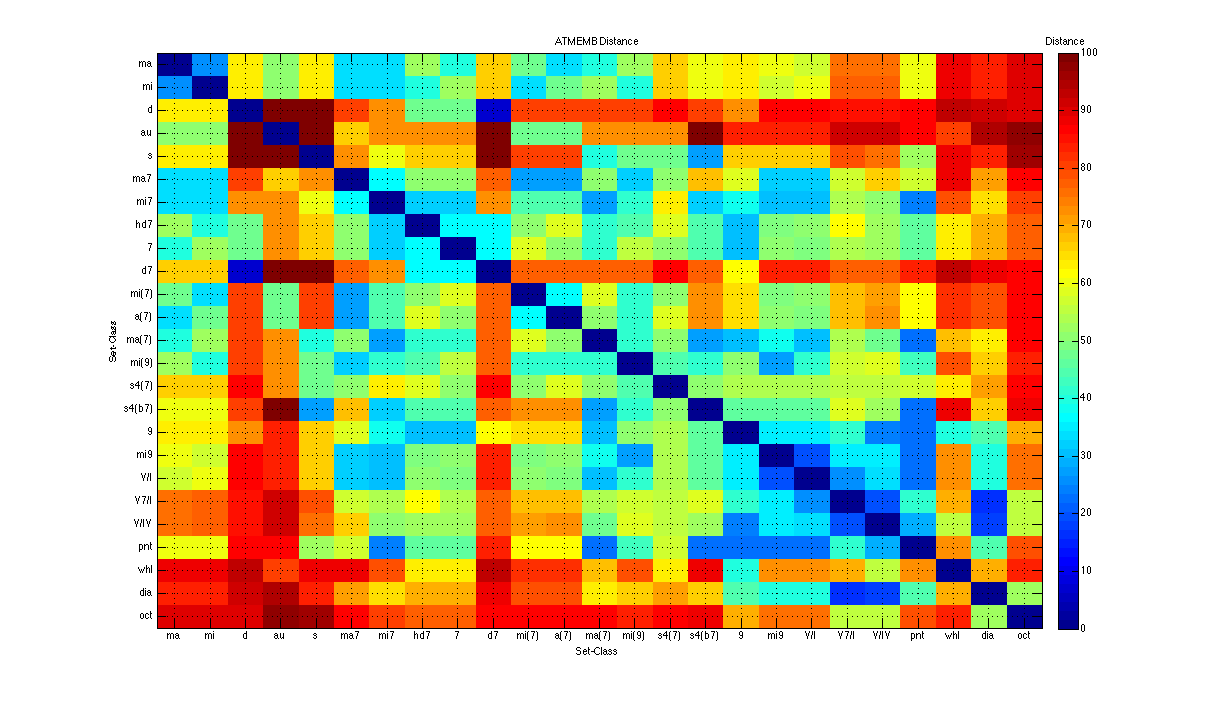
\includegraphics[width=.9\linewidth]{../plots/ATMEMB_chord_comparison.png}
\caption{\label{fig:atmembchordcomp}ATMEMB distance between tonal objects}
\end{figure}
\begin{figure}[htb]
\centering
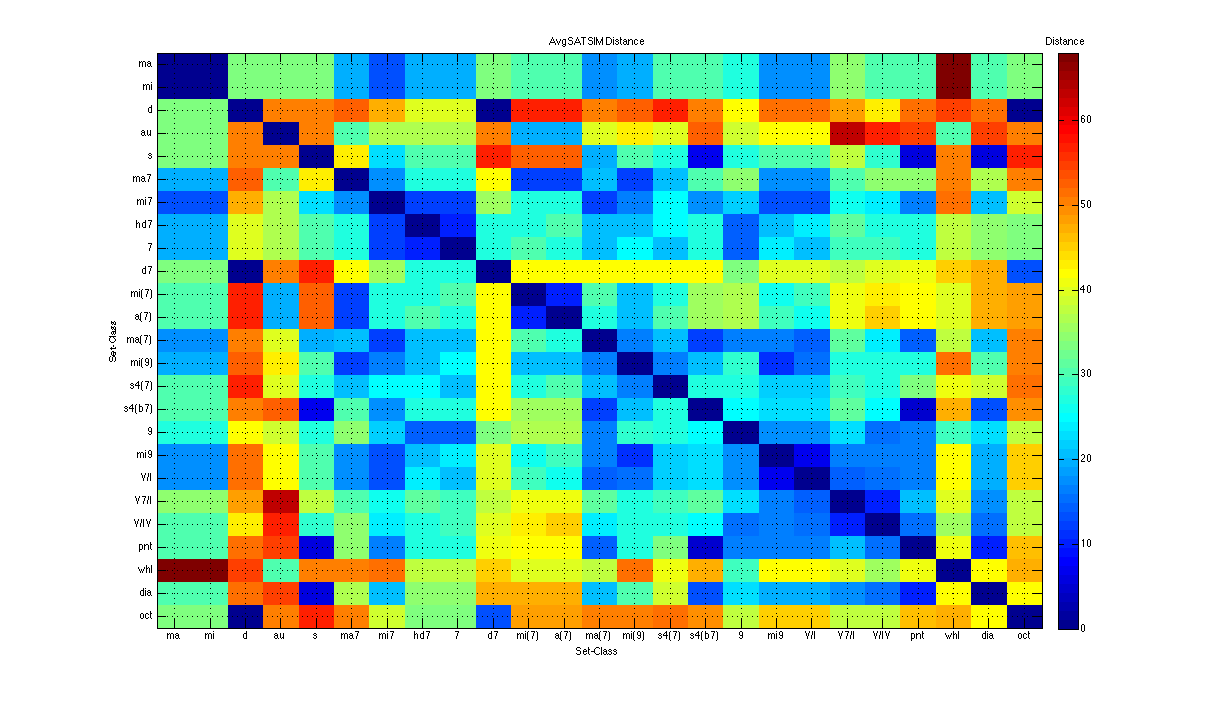
\includegraphics[width=.9\linewidth]{../plots/AvgSATSIM_chord_comparison.png}
\caption{\label{fig:avgsatsimchordcomp}AvgSATSIM distance between tonal objects}
\end{figure}

As can be seen, the values for these chord types are quite dissimilar
for the different measures. Thus, measure selection will be an
inportant part of the analysis depending on their specific
discriminatory power. Therefore, these plots willform a useful
reference guide when selecting parameters and values for the
visualisation techniques described in Chapter \ref{sec-9}.
\subsection{Total Measure Comparison}
\label{sec-7-8}

For a more quantitative comparison of the measures, the absolute
difference between corresponding values can be calculated and ploted
on similar grids. This gives an overall visualisation of where the
measures most disagree. Figure \ref{fig:absdiff} shows a matrix of
plots each comparing the values of two measures. Each plot displays
only half the table as the they are symmetric. The lighter blue and
green areas indicate higher discrepancy between the measures' values.

\begin{figure}[htb]
 \centering
 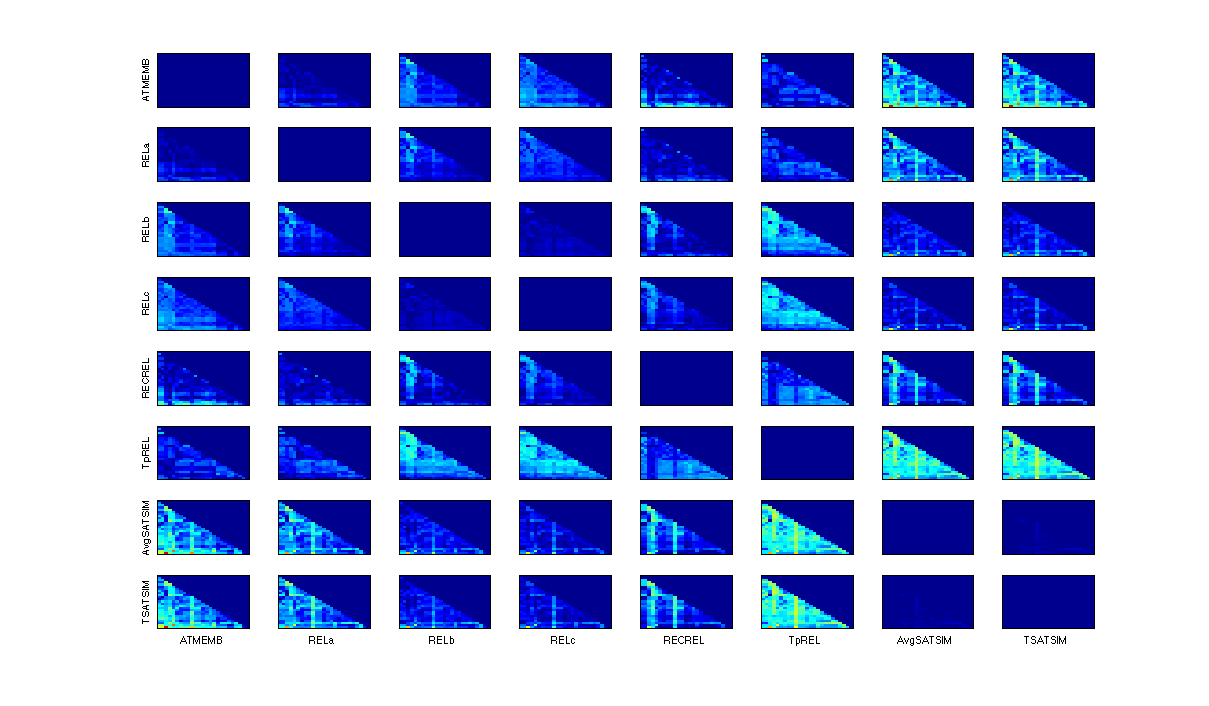
\includegraphics[width=.9\linewidth]{../plots/Measure_comparisons.png}
 \caption{\label{fig:absdiff}Absolute difference between measures' values}
 \end{figure} 

A more compact representation of these comparisons can be obtained by
correlation of the vectors containing the values from each
measure. Figure \ref{fig:measurecorrchords} shows a grid where each
square corresponds to the comparison between two measures and is
coloured according the correlation of the values for the common chord
types. For the purposes of comparison, Figure \ref{fig:measurecorrall}
shows a similar plot to Figure \ref{fig:measurecorrchords} but rather
displays the correlation involving all the 61425 pairwise Tn-type SC
comparisons for each measure.

\begin{figure}[htb]
\centering
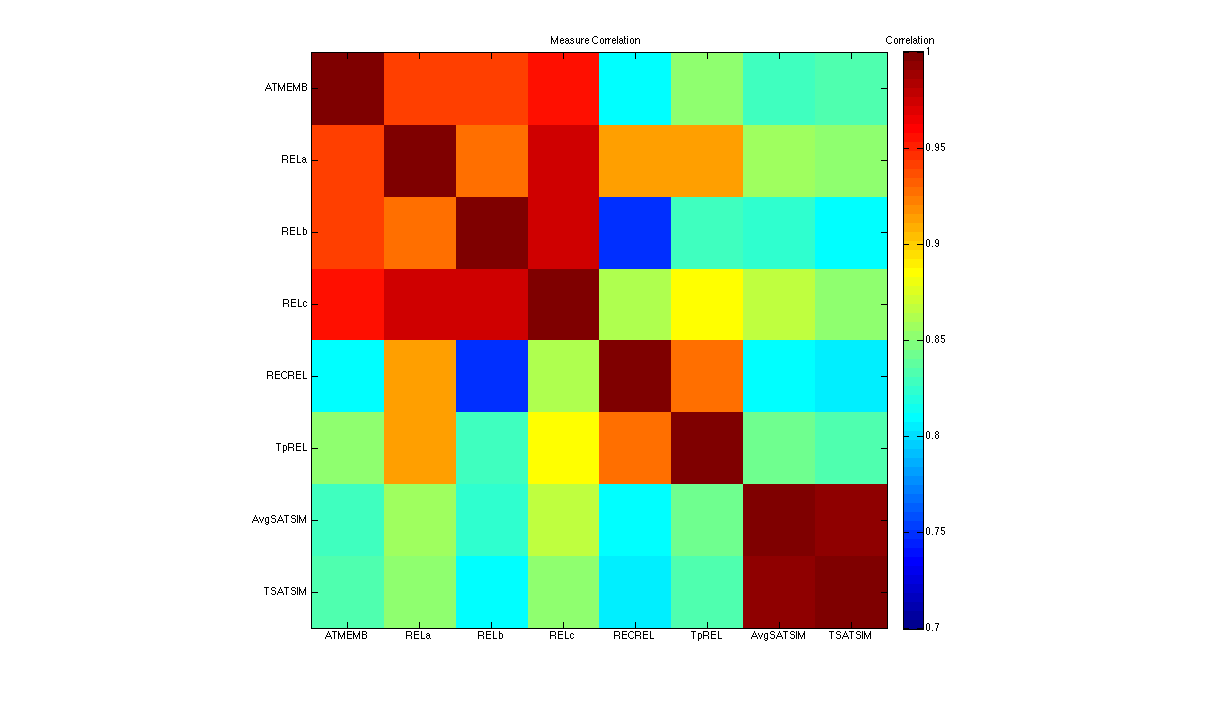
\includegraphics[width=.9\linewidth]{../plots/Measure_Correlation.png}
\caption{\label{fig:measurecorrchords}Correlation between measures' values for common chords}
\end{figure}

\begin{figure}[htb]
\centering
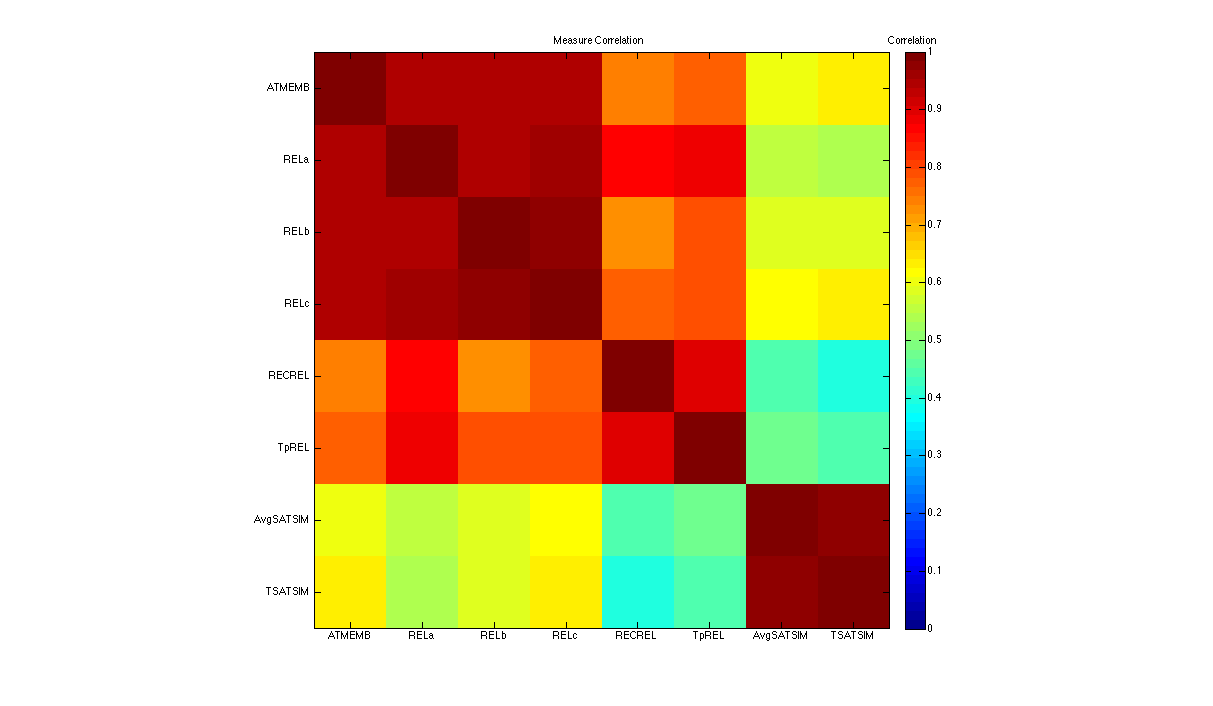
\includegraphics[width=.9\linewidth]{../plots/Measure_Correlation_All.png}
\caption{\label{fig:measurecorrall}Correlation between measures' values for all SCs}
\end{figure}
\subsection{Chapter Conclusions}
\label{sec-7-9}

\begin{itemize}
\item general comments about measure discrimination?
\begin{itemize}
\item high/low
\item major minor
\item cardinality
\item symmetric sets
\item inversionally related sets
\end{itemize}
\item these plots will aid selection of comparison sets
\item abs diff plot
\begin{itemize}
\item which measures are closest
\item avgsatsim - tsatsim
\item which measures are furthest
\item closer inspection
\end{itemize}
\item chord corr plot
\begin{itemize}
\item measures tend to agree
\item most different measures
\item recrel - relb: why?
\end{itemize}
\item SC corr plot
\begin{itemize}
\item means of comparison
\item common chord types have common properties that the measures tend
    to treat in a similar way.
\end{itemize}
\item repertiore
\begin{itemize}
\item what repertoire contains what chords
\item billboard
\item beatles
\end{itemize}
\end{itemize}
\section{Segmentation}
\label{sec-8}

As mentioned in \ref{sec-3-6}, segmentation is a very
important stage of the analysis. The segmentation policy used strongly
influeces the SC content that can be observed, with larger segments
tending to contain higher cardinality sets. Using a sliding window to
segment the music requires careful consideration of the specific
window length and hop size depending not only on the type and
cardinality of sets that the analyst desires to observe but also on
the way in which the data will then be visualised.

In this chapter we outline two segmentation policies:
\begin{enumerate}
\item A sliding window with fixed length and hopsize.
\item The systematic segmentation policy of \citet{Martorell2013}.
\end{enumerate}
\subsection{Systematic Segmentation}
\label{sec-8-1}

\citet[chap. 5.3]{Martorell2013} specifies a fully systematic
segmentation policy which exhaustivly records every change in the PC
material of a piece. The segments are of variable length but together
capture the entire SC contents of the music. With each segment indexed
in time by its center, the data structure, known as a cass-scape, is a
sparse 3-dimensional binary matrix with axes representing time,
time-scale (segment length) and set class. 

\citet[chap. 5.3.5]{Martorell2013} specifies two compact
representations of this data as a means of observing the the global SC
content of a piece.

Class-matrix: The class-matrix is a 2d projection the class-scape
obtained by removing the time-scale information. This, in effect, acts
to expand each point to the actual duration of the segment it
represents.

Class-vector: The class-vector is a further reduction of data showing
the relative active duration of each class in the class-matrix and is
expressed as a percentage of the total duration of the piece.

The systematic segmentation policy was applied to a MIDI
representation of the C major Prelude from Book 1 of The Well Tempered
Clavier by Bach. Figures \ref{fig:classmat} and \ref{fig:classvec}
show the class-matrix and class-vector respectively for the Bach
prelude.

\begin{figure}[htb]
\centering
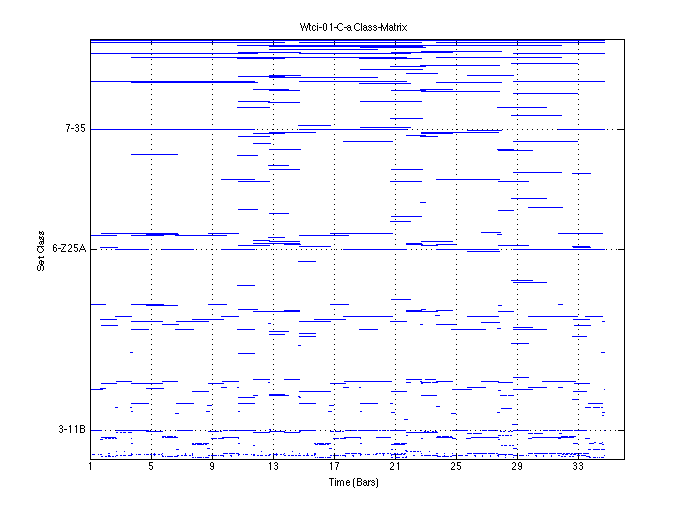
\includegraphics[width=.9\linewidth]{../plots/classmat.png}
\caption{\label{fig:classmat}Class-matrix for Bach WTCi Prelude 1}
\end{figure}
\begin{figure}[htb]
\centering
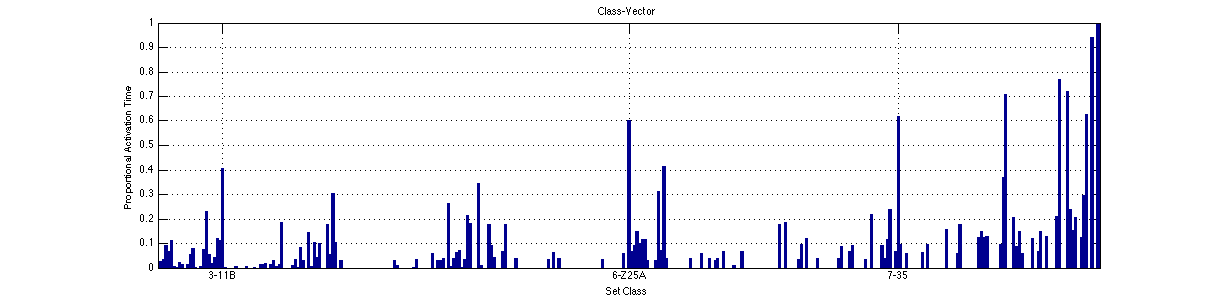
\includegraphics[width=.9\linewidth]{../plots/classvec.png}
\caption{\label{fig:classvec}Class-vector for Bach WTCi Prelude 1}
\end{figure}

\begin{itemize}
\item What do they show?
\begin{itemize}
\item a profile of the sc contents
\end{itemize}
\item bach victoria diatoniscm
\end{itemize}

From this complete information it is also possible to view statistical
information about which SCs or type of SCs appear in which time
scale. Figure \ref{fig:avgseglengthsc} plots the average segment
length and standard deviation for each SC. Figure
\ref{fig:avgseglengthcard} shows the same information for each
cardinality class.

\begin{figure}[htb]
\centering
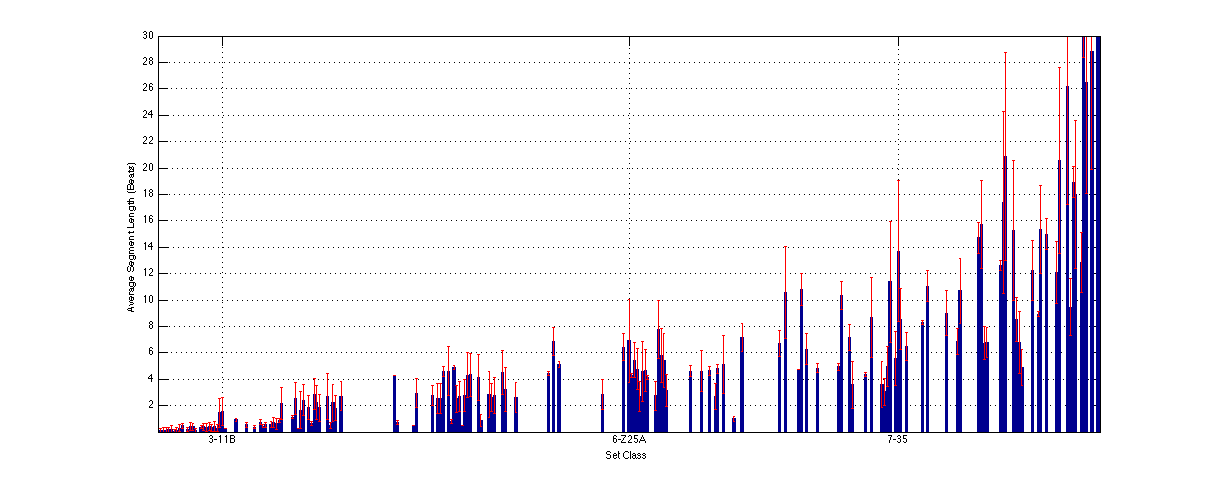
\includegraphics[width=.9\linewidth]{../plots/avgseglengthsc.png}
\caption{\label{fig:avgseglengthsc}Average segment length and STD for each SC in Bach WTCi Prelude 1}
\end{figure}

\begin{figure}[htb]
\centering
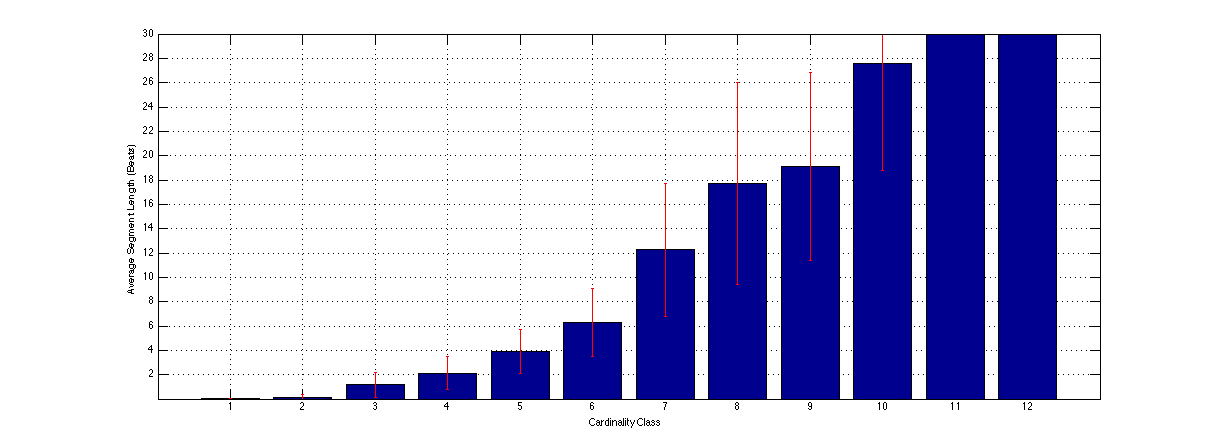
\includegraphics[width=.9\linewidth]{../plots/avgseglengthcard.png}
\caption{\label{fig:avgseglengthcard}Average Segment length and STD for each nC in Bach WTCi Prelude 1}
\end{figure}
\subsection{Sliding Window}
\label{sec-8-2}

Segmentation using a sliding window with fixed window and hop size is
used to obtain an SC time series of one specific time-scale. This time
series is then used for the visualisation techniques outlined in the
next chapter. The purpose of the sliding window is to allow the
analyst to focus on particular sets or tune in to one particular
cardinality. This tuning process is performed through selection of an
appropriate window and hop size. The selection of window and hop size
can be informed by exploration of the data obtained from the
systematic segmentation.

For example, from Figure \ref{fig:avgseglengthcard} in the previous
section it can be seen that three note chords have an average window
length of XXXXX. Specifically, from Figure \ref{fig:avgseglengthsc},
major chords (3-11B) have an average window length of XXXXX. Figure
\ref{fig:cvplusswseg} displays the results of a sliding window
segmentation of the piece with a window size of XXXX and hop size of
XXXXX. The SC contents extracted from this segmentation are displayed
in red on top of the class-vector. This representation gives an
indication of what proportion of the overall class contents have been
retrieved by the sliding window segmentation.

\begin{figure}[htb]
\centering
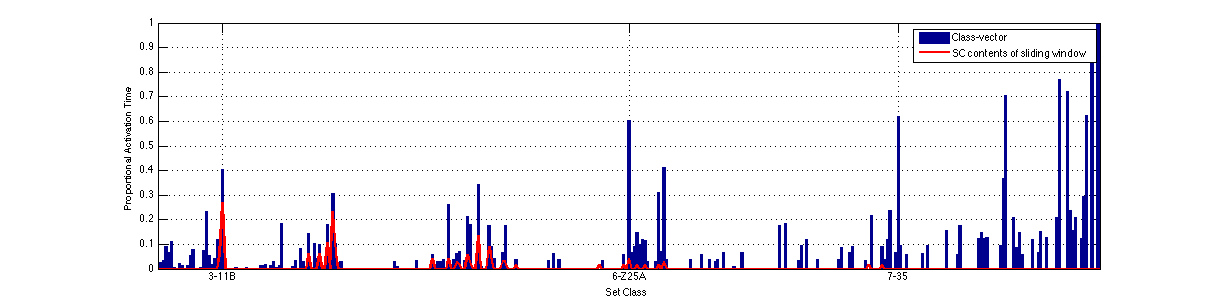
\includegraphics[width=.9\linewidth]{../plots/classvecclasshist.png}
\caption{\label{fig:cvplusswseg}SC contents from sliding window segmentation (red) superimposed on class-vector (black)}
\end{figure}

The plot shows that the particular segmentation policy has captured a
higher proportion of SC 3-11B than other types. This specific
targeting of SCs will be exploited in the visualisation techniques
described in \ref{sec-9}.
\section{Visualisation}
\label{sec-9}

This chapter outlines three visualisation techniques that may be used
in conjunction to represent SC class information of a musical piece so
as to retrieve meaningful analysis.
\subsection{Distance Plot}
\label{sec-9-1}

The distance plot provides a simple means of capturing how the pitch
content of a piece evolves in time with respect to a specific SC. It
involves segmenting the piece using a fixed sliding window and
calculating the distance between each segment and a comparison set.

There are three interdependent parameters which must be selected
according to the specific intentions of the analyst: Segmentation
(window and hop size), comparison set and similarity/distance
measure. The segmentation determines the captured SC content which
should be targeted according to its relationship to the comparison
set. This relationship is determined by the measure used which must
possess an adequate degree of discrimination so as to produce
noticable changes in the time series.

Figure \ref{fig:distplot} shows an example distance time series
plotted in as a line for the Bach Prelude. The same sliding window
segmentation as Figure \ref{fig:cvplusswseg} was used so as to capture
three note chords, specifically major chords (3-11B). Each segment was
compared to SC 3-11B using the ATMEMB-prime distance.

\begin{figure}[htb]
\centering
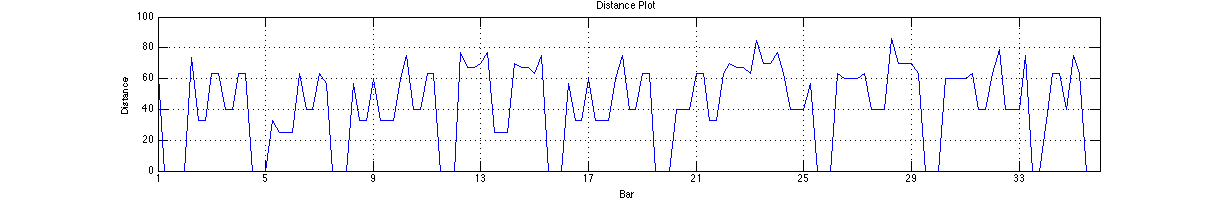
\includegraphics[width=.9\linewidth]{../plots/distplot.png}
\caption{\label{fig:distplot}ATMEMB-prime distance plot (3-11B)}
\end{figure}

As Figure \ref{fig:cvplusswseg} indicates a higher proportion of SC
3-11B present in the segments, it is unsurprising to see the line
frequently displaing a distance of 0 where the segment coincides with
the comparison set. A plot such as this gives an indication as to the
tonal progression of the piece, indicatind where the sonority most
resembles that of a simple major triad. Higher parts of the curve
indicate more complicated or less familiar harmonic passages.

\begin{itemize}
\item different measures
\item different comparison sets
\end{itemize}
\subsection{Auto-correlation}
\label{sec-9-2}

The distance plots described in the previous section can give a basic
view of the tonal progression of a piece. In many cases they contain
recurring patterns where passages with similar SC content producing
similar curves. A further visualisation technique is
autocorrelation. By autocorrelating the distance plot it may be
possible to capture some structural elements of the piece. The
autocorrelation time series will contain peaks corresponding to
``similar'' passages. For example, an piece with a structure of A-B-A
will have an autocorrelation plot with a slight peak corresponding to
beginning of the repeat of section A.

Figure \ref{fig:autocorr} shows the autocorrelation function of the
distance plot in Figure \ref{fig:distplot}. The peaks that appear at
regular intervals correspond to repeticions of particular tonal
sequences in the piece.

\begin{figure}[htb]
\centering
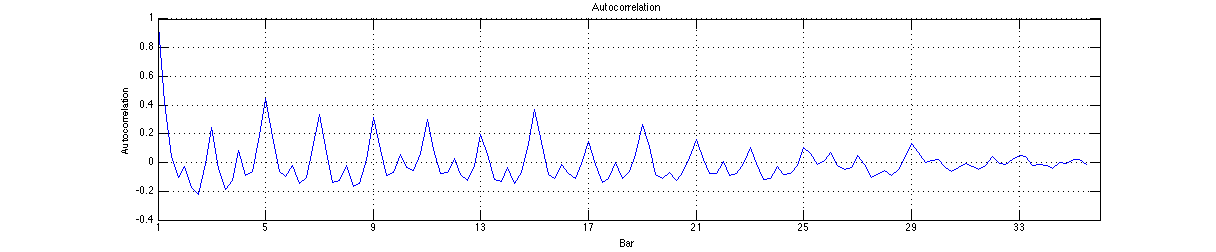
\includegraphics[width=.9\linewidth]{../plots/autocorr.png}
\caption{\label{fig:autocorr}Autocorrelation of distance plot}
\end{figure}
\subsection{Self-similarity matrix}
\label{sec-9-3}

As an alternative to using a specific comparison set, the distance of
a segment to other segments in the piece could be observed. A
systematic way of doing this is computing the self-similarity matrix
which provides a simples means for descovery of repetitions in a time
series. The patterns present in a visualisation of a self-similarity
matrix can indicate similar passages and structural elements of a
piece.

Figure \ref{fig:selfsimmat} shows the self-similarity matrix computed
from the sliding window SC time-series. The diagonal line highlighted
in red represents the repetition of a four bar sequence: bars 5-11 in
the tonic key are repeated in bars 15-19 with a transposition to the
dominant key.

\begin{figure}[htb]
\centering
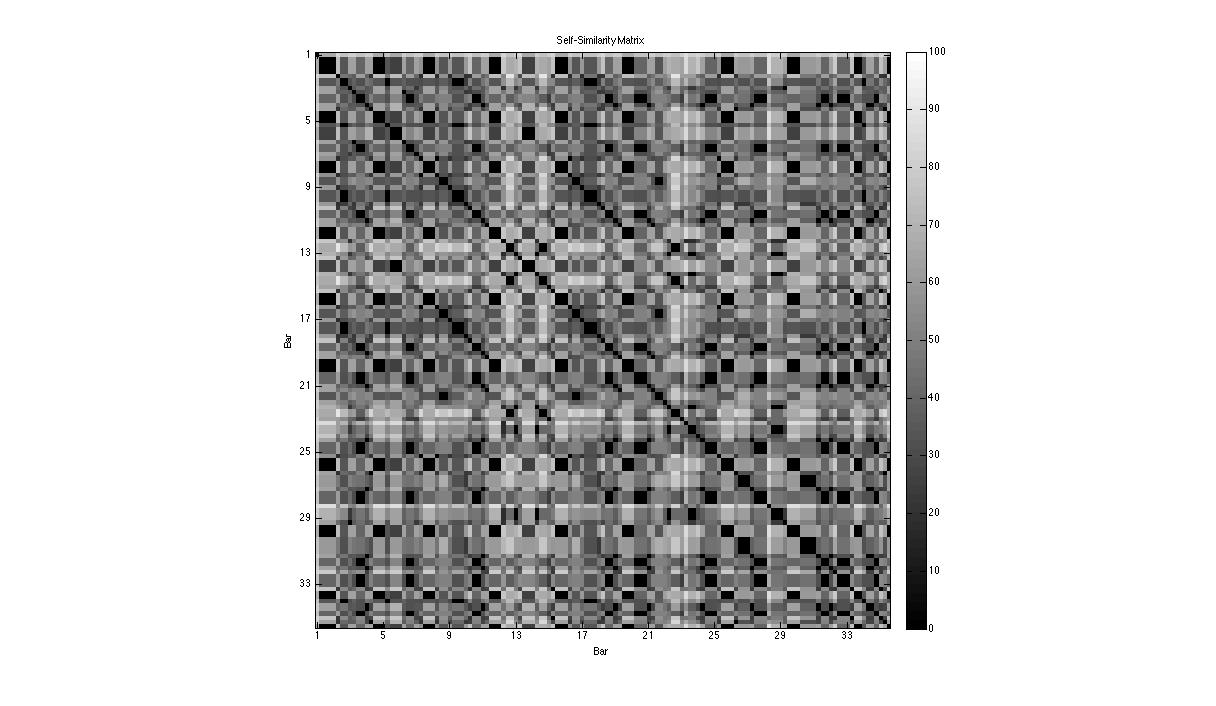
\includegraphics[width=.9\linewidth]{../plots/selfsimmat.png}
\caption{\label{fig:selfsimmat}Self-similarity matrix of SC time series}
\end{figure}
\subsection{Conclusions}
\label{sec-9-4}

\begin{itemize}
\item 
\end{itemize}
\section{Analysis Tool}
\label{sec-10}

\begin{itemize}
\item Due to the complex relationship between the selection of the various
  parameters involved in this kind of analysis, it is desireable to
  work in an interactive and exploratory environment.
\item for exploratory analysis
\end{itemize}
\section{MDS}
\label{sec-11}

\begin{itemize}
\item Visualisation of values using MDS
\item r2 against stress for different measures
\item comparison
\item visualisation
\end{itemize}
\section{Conclusions}
\label{sec-12}
\section{Future Work}
\label{sec-13}

\begin{itemize}
\item 
\end{itemize}
\section{Latex Stuff}
\label{sec-14}

\clearpage
\bibliographystyle{plainnat}
\bibliography{/Users/nick/Documents/MendeleyDesktop/library.bib}

\clearpage
\appendix
\section{SC Similarity Measures}
\label{sec-15}

This chapter contains a concise summary of the SC similarity measures
from the literature organised by theorist. Each section specifies the
publication in which the measure was proposed and brief description of
the theoretical approach adopted by the theorist. A mathmatical
formula is given where possible using standard notation. A reference
for notation can be found in \ref{sec-3-3-4} and commonly used symbols are
defined in the glossary. Where a mathematical formula does suffice,
the comparison proceedure is described in words. In addition, each
section contains a table specifying important statistics:
\begin{itemize}
\item SC-Type: the type of SC the measure compares (Tn or TnI)
\item Cardinality: whether the measure can compare SCs of different
  cardinalities.
\item Vector Type: the type of vector used in the comparison procedure
  (see \ref{sec-3-3}).
\item Max Similarity: the value that indicates maximum similarity from all
  possible comparisons.
\item Min Similarity: the value that indicates minimum similarity from all
  possible comparisons.
\item Average Value: the average value from all possible comparisons.
\item No. Values: the number of distinct values produced from all possible
  comparisons.
\item Criteria Met: a list of Castren's criter which the measure meets.
\item I-related: whether the measure descriminates between inversionally
  related sets.
\item Z-related: whether the measure discriminated between Z-related sets.
\end{itemize}
\subsection{MORRIS}
\label{sec-15-1}
\subsubsection{K}
\label{sec-15-1-1}

Presented in \citet[pp. 448]{Morris1979}, the K measure gives the
number of intervals-classes (dyad-classes) shared by two SCs, X and Y.
$$ K(X,Y)= \sum_{i=1}^{6}{MIN(x_{i},y_{i})} $$

\begin{center}
\begin{tabular}{ll}
 SC Type:         &  TnI                 \\
 Cardinality:     &  Any                 \\
 Vector Type:     &  ICV                 \\
 Max Similarity:  &  55                  \\
 Min Similarity:  &  0                   \\
 Average Value:   &  10                  \\
 No. Values:      &  35                  \\
 Criteria Met:    &  C1,C2,C3.3,C3.4,C4  \\
 I-related:       &  No                  \\
 Z-related:       &  No                  \\
\end{tabular}
\end{center}


\begin{itemize}
\item Problems: scale of values not the same for all value groups.
\end{itemize}
\subsubsection{SIM}
\label{sec-15-1-2}

Presented in \citet[pp. 446]{Morris1979}, SIM compares the ICVs of
two SCs (the value is the cardinality of the DV).
$$SIM\left(X,Y\right)=\sum_{i=1}^{6}\left|x_{i}-y_{i}\right|$$
or
$$SIM\left(X,Y\right)=\#DV\left(ICV\left(X\right),ICV\left(Y\right)\right)$$
SIM is a function of K:
$$SIM(X,Y) = \#ICV(X) + \#ICV(Y) - 2.K(X,Y)$$

\begin{center}
\begin{tabular}{ll}
 SC Type:         &  TnI                 \\
 Cardinality:     &  Any                 \\
 Vector Type:     &  ICV                 \\
 Max Similarity:  &  0                   \\
 Min Similarity:  &  65                  \\
 Average Value:   &  13                  \\
 No. Values:      &  44                  \\
 Criteria Met:    &  C1,C2,C3.3,C3.4,C4  \\
 I-related:       &  No                  \\
 Z-related:       &  No                  \\
\end{tabular}
\end{center}


\begin{itemize}
\item Problems: scale not the same for all value groups. course resolution
  when cardinalities differ greatly
\end{itemize}
\subsubsection{ASIM}
\label{sec-15-1-3}

Presented in \citet[pp. 450]{Morris1979}, ASIM (Absolute SIM) is a
scaled version of SIM to address criteria C3.1.
$$ASIM\left(X,Y\right)=\frac{SIM\left(X,Y\right)}{\#ICV\left(X\right)+\#ICV\left(Y\right)}$$

\begin{center}
\begin{tabular}{ll}
 SC Type:         &  TnI                      \\
 Cardinality:     &  Any                      \\
 Vector Type:     &  ICV                      \\
 Max Similarity:  &  0                        \\
 Min Similarity:  &  1                        \\
 Average Value:   &  0.42                     \\
 No. Values:      &  79                       \\
 Criteria Met:    &  C1,C2,C3.1,C3.2,C3.4,C4  \\
 I-related:       &  No                       \\
 Z-related:       &  No                       \\
\end{tabular}
\end{center}


Problems: Fixed the scale of values, but still coarse resolution when
cardinalities differ greatly. Scaling is done as the last step.
\subsection{LORD}
\label{sec-15-2}
\subsubsection{sf}
\label{sec-15-2-1}

Presented in \cite[pp. 93]{Lord1981}, sf (Similarity Function) is
similar to SIM but developed independently. sf is a subset of SIM:
$$sf\left(X,Y\right)=\frac{\#DV\left(ICV\left(X\right),ICV\left(Y\right)\right)}{2}=\frac{SIM(X,Y)}{2}$$

\begin{center}
\begin{tabular}{ll}
 SC Type:         &  TnI           \\
 Cardinality:     &  Same          \\
 Vector Type:     &  ICV           \\
 Max Similarity:  &  0             \\
 Min Similarity:  &  9             \\
 Average Value:   &  3             \\
 No. Values:      &  10            \\
 Criteria Met:    &  C3.3,C3.4,C4  \\
 I-related:       &  No            \\
 Z-related:       &  No            \\
\end{tabular}
\end{center}
\subsection{TEITELBAUM}
\label{sec-15-3}
\subsubsection{s.i.}
\label{sec-15-3-1}

Presented in \citet[pp. 88]{Teitelbaum1965}, s.i. (Similarity Index)
is the Euclidean distance between the carteasian coordinates defined
by the ICVs of two SCs. This is equivelant to the magnitude of the
difference vector.
$$s.i.(X,Y)=\sqrt{\sum_{i=1}^{6}(x_{i}-y_{i})^{2}}=\left\|DV(ICV(X),ICV(Y))\right\|$$

\begin{center}
\begin{tabular}{ll}
 SC Type:         &  TnI        \\
 Cardinality:     &  Same       \\
 Vector Type:     &  ICV        \\
 Max Similarity:  &  1.41       \\
 Min Similarity:  &  8.49       \\
 Average Value:   &  2.85       \\
 No. Values:      &  31         \\
 Criteria Met:    &  C3.3,C3.4  \\
 I-related:       &  No         \\
 Z-related:       &  No         \\
\end{tabular}
\end{center}


\begin{itemize}
\item Same cardinality only
\item Z-related sets not compared
\end{itemize}
\subsection{ROGERS}
\label{sec-15-4}
\subsubsection{IcVD$_{1}$}
\label{sec-15-4-1}

Presented in \citet{Rogers1992}, IcVD$_{1}$ (Distance Formula 1) is a
modification of SIM (\ref{sec-15-1-2}). The ICV components are scaled before being
summed. IcVD$_{1}$ is related to Castren's \%REL$_{2}$ (\ref{sec-15-8-3}):
\%REL$_{2}$(X,Y) = IcVD$_{1}$(X,Y)\texttimes{} 50.  

$$IcVD_{1}(X,Y)=\#DV\left(\frac{ICV(X)}{\#ICV(X)},\frac{ICV(Y)}{\#ICV(Y)}\right)$$


\begin{center}
\begin{tabular}{ll}
 SC Type:         &  TnI                      \\
 Cardinality:     &  Any                      \\
 Vector Type:     &  ICV                      \\
 Max Similarity:  &  0                        \\
 Min Similarity:  &  2                        \\
 Average Value:   &  0.59                     \\
 No. Values:      &  140                      \\
 Criteria Met:    &  C1,C2,C3.1,C3.2,C3.4,C4  \\
 I-related:       &  No                       \\
 Z-related:       &  No                       \\
\end{tabular}
\end{center}
\subsubsection{IcVD$_{2}$}
\label{sec-15-4-2}

Presented in \citet{Rogers1992}, IcVD$_{2}$ (Distance Formula 2) is
similar to s.i. (\ref{sec-15-3-1}), but instead returns the Euclidean distance
between the ends of the normalised ICVs.
$$IcVD_{2}(X,Y)=\left\|DV(\hat{ICV(X)},\hat{ICV(Y)})\right\|$$

\begin{center}
\begin{tabular}{ll}
 SC Type:         &  TnI                   \\
 Cardinality:     &  Any                   \\
 Vector Type:     &  ICV                   \\
 Max Similarity:  &  0                     \\
 Min Similarity:  &  1.41                  \\
 Average Value:   &  0.54                  \\
 No. Values:      &  133                   \\
 Criteria Met:    &  C1,C2,C3.1,C3.2,C3.4  \\
 I-related:       &  No                    \\
 Z-related:       &  No                    \\
\end{tabular}
\end{center}


\begin{itemize}
\item Problems: does not produce uniform values for comparable cases
\end{itemize}
\subsubsection{Cos($\theta$)}
\label{sec-15-4-3}

Presented in \citet{Rogers1992}, Cos$\theta$, gives the cosine of the
angle between the ICVs in six-dimensional euclidean space. As the
angle decreases the similarity approaches 1.
$$Cos\theta(X,Y)=\frac{ICV(X)\cdot ICV(Y)}{\left\|ICV(X)\right\|\times\left\|ICV(Y)\right\|}$$

\begin{center}
\begin{tabular}{ll}
 SC Type:         &  TnI                   \\
 Cardinality:     &  Any                   \\
 Vector Type:     &  ICV                   \\
 Max Similarity:  &  1                     \\
 Min Similarity:  &  0                     \\
 Average Value:   &  0.81                  \\
 No. Values:      &  92                    \\
 Criteria Met:    &  C1,C2,C3.1,C3.2,C3.4  \\
 I-related:       &  No                    \\
 Z-related:       &  No                    \\
\end{tabular}
\end{center}


\begin{itemize}
\item Problems: C4
\end{itemize}
\subsection{RAHN}
\label{sec-15-5}
\subsubsection{AK}
\label{sec-15-5-1}

Presented in /citet[pp. 489]\{Rahn1979\}, AK is an absolute or adjusted
version of Morris' K (\ref{sec-15-1-1}), addressing the C3.1 criteria. AK is related
to Morris' ASIM: AK(X,Y)=1-ASIM(X,Y).
$$AK\left(X,Y\right)=\frac{2K\left(X,Y\right)}{\#ICV\left(X\right)+\#ICV\left(Y\right)}$$

\begin{center}
\begin{tabular}{ll}
 SC Type:         &  TnI                      \\
 Cardinality:     &  Any                      \\
 Vector Type:     &  ICV                      \\
 Max Similarity:  &  1                        \\
 Min Similarity:  &  0                        \\
 Average Value:   &  0.58                     \\
 No. Values:      &  78                       \\
 Criteria Met:    &  C1,C2,C3.1,C3.2,C3.4,C4  \\
 I-related:       &  No                       \\
 Z-related:       &  No                       \\
\end{tabular}
\end{center}


\begin{itemize}
\item Problems: single scale of values (C4), but poor discrimination for
  some value groups.
\end{itemize}
\subsubsection{MEMB$_{n}$}
\label{sec-15-5-2}

Presented in \citet[pp. 492]{Rahn1979}, MEMB$_{n}$ (Mutual Embedding
Number) compares the nCVs of two SCs for one nC at a time. It meausres
the mutual embedding of subsets such that only non-zero components of
the nCVs contribute. By setting n = 2 (MEMB$_{2}$) it compares ICVs.
$$MEMB_{n}\left(X,Y\right)=\sum_{i=1}^{\#nC}{nCV(X)_{i}+nCV(Y)_{i}}$$
such that nCV(X)$_{i}$>0 and nCV(Y)$_{i}$>0. 

\begin{center}
\begin{tabular}{ll}
 SC Type:         &  TnI or Tn           \\
 Cardinality:     &  Any                 \\
 Vector Type:     &  nCV                 \\
 Max Similarity:  &  121                 \\
 Min Similarity:  &  0                   \\
 Average Value:   &  30                  \\
 No. Values:      &  79                  \\
 Criteria Met:    &  C1,C2,C3.3,C3.4,C4  \\
 I-related:       &  Yes*                \\
 Z-related:       &  Yes*                \\
\end{tabular}
\end{center}


\begin{itemize}
\item Problems: does not produce uniform scale of values for all value
  groups.
\end{itemize}
\subsubsection{TMEMB}
\label{sec-15-5-3}

Presented in \citet[pp. 492]{Rahn1979}, TMEMB (Total Mutual Embedding
Number) counts the mutually embedded subsets of every
cardinality. TMEMB is a total measure.
$$TMEMB\left(X,Y\right)=\sum_{n=2}^{12}MEMB_{n}\left(X,Y\right)$$

\begin{center}
\begin{tabular}{ll}
 SC Type:         &  TnI or Tn         \\
 Cardinality:     &  Any               \\
 Vector Type:     &  nCV               \\
 Max Similarity:  &  6118              \\
 Min Similarity:  &  0                 \\
 Average Value:   &  131               \\
 No. Values:      &  877               \\
 Criteria Met:    &  C1,C2,C3.3,C4,C5  \\
 I-related:       &  Yes               \\
 Z-related:       &  Yes               \\
\end{tabular}
\end{center}


\begin{itemize}
\item Problems: Different value scales for different value groups
\end{itemize}
\subsubsection{ATMEMB}
\label{sec-15-5-4}

Presented in \citet[pp. 494]{Rahn1979}, ATMEMB (Adjusted Total Mutual
Embedding Number) is a scaled version of TMEMB to address criteria
C3.1 (like SIM and ASIM; A and AK). ATMEMB is a total measure.
$$ATMEMB\left(X,Y\right)=\frac{TMEMB\left(X,Y\right)}{2^{\#X}+2^{\#Y}-\left(\#X+\#Y+2\right)}$$

\begin{center}
\begin{tabular}{ll}
 SC Type:         &  TnI or Tn                   \\
 Cardinality:     &  Any                         \\
 Vector Type:     &  nCV                         \\
 Max Similarity:  &  1                           \\
 Min Similarity:  &  0                           \\
 Average Value:   &  0.45                        \\
 No. Values:      &  101                         \\
 Criteria Met:    &  C1,C2,C3.1,C3.2,C3.4,C4,C5  \\
 I-related:       &  Yes                         \\
 Z-related:       &  Yes                         \\
\end{tabular}
\end{center}
\subsection{ISAACSON}
\label{sec-15-6}
\subsubsection{AMEMB2}
\label{sec-15-6-1}

Proposed by \citet[pp. 8]{Isaacson1990}, AMEMB$_{2}$ (Adjusted MEMB$_{2}$)
is a scaled version MEMB$_{2}$ (\ref{sec-15-5-2}), measuring the mutual
embedding of ICs.

$$AMEMB_{2}=\frac{2 \times
MEMB_{2}(X,Y)}{\left(\#X\left(\#X-1\right)+\#Y\left(\#Y-1\right)\right)}$$

\begin{center}
\begin{tabular}{ll}
 SC Type:         &  TnI  \\
 Cardinality:     &  Any  \\
 Vector Type:     &  ICV  \\
 Max Similarity:  &  1    \\
 Min Similarity:  &  0    \\
 Average Value:   &       \\
 No. Values:      &       \\
 Criteria Met:    &       \\
\end{tabular}
\end{center}
\subsubsection{IcVSIM}
\label{sec-15-6-2}

Presented in \citet[pp. 18]{Isaacson1990}, IcVSIM (Interval-Class
Vector Similarity Relation) is the standard deviation of the entries
in the ICVs of two SCs. IcVSIM is a scaled version of
s.i. (\ref{sec-15-3-1}). IdV$_{i}$ is the ith term in the vector defined by
ICV(X)-ICV(Y) and $\overline{DV}$ is the average (mean) of its
entries.
$$IcVSIM(X,Y)=\sqrt{\frac{\sum(IdV_{i}-\overline{IdV})^{2}}{6}}$$

\begin{center}
\begin{tabular}{ll}
 SC Type          &  TnI         \\
 Cardinality:     &  Any         \\
 Vector Type:     &  ICV         \\
 Max Similarity:  &  0           \\
 Min Similarity:  &  3.64        \\
 Average Value:   &  1.2         \\
 No. Values:      &  121         \\
 Criteria Met:    &  C1,C2,C3.4  \\
 I-related:       &  No          \\
 Z-related:       &  No          \\
\end{tabular}
\end{center}
\subsubsection{ISIM2}
\label{sec-15-6-3}

Presented in \citet{Isaacson1996}, ISIM2 is a scaled version of IcVSIM
(\ref{sec-15-6-2}). The squre root is taken of each term in the ICVs. Isaacson
argues that each additional instance of an IC contributes less to
similitude. However, \citet{Samplaski2005a} found ISIM2 to be
inconsistent with itself when applying MDS to the values produced.

\begin{center}
\begin{tabular}{ll}
 SC Type          &  TnI         \\
 Cardinality:     &  Any         \\
 Vector Type:     &  ICV         \\
 Max Similarity:  &              \\
 Min Similarity:  &              \\
 Average Value:   &              \\
 No. Values:      &              \\
 Criteria Met:    &  C1,C2,C3.4  \\
\end{tabular}
\end{center}
\subsubsection{ANGLE (Isaacson \& Scott)}
\label{sec-15-6-4}

\citet{Scott1998} propose a geometric method which is identical to
that of Cos/theta (\ref{sec-15-4-3}) but instead gives the size of the
angle in degrees. $$ANGLE(X,Y) = \arccos{Cos\theta(X,Y)}$$

\begin{center}
\begin{tabular}{ll}
 SC Type          &  TnI                   \\
 Cardinality:     &  Any                   \\
 Vector Type:     &  ICV                   \\
 Max Similarity:  &                        \\
 Min Similarity:  &                        \\
 Average Value:   &                        \\
 No. Values:      &                        \\
 Criteria Met:    &  C1,C2,C3.1,C3.2,C3.4  \\
 I-related:       &  No                    \\
 Z-related:       &  No                    \\
\end{tabular}
\end{center}
\subsection{LEWIN}
\label{sec-15-7}
\subsubsection{REL}
\label{sec-15-7-1}

Presented in \citet{Lewin1979}, REL compares the nCVs of two SCs for
all the nCs. Like MEMB$_{n}$ (\ref{sec-15-5-2}), REL only considers non-zero
entries however, this is achieved by multiplication (taking the
geometric mean) of corresponding nCV terms.

$$REL(X,Y)=\frac{\sum_{i=1}^{p}{\sqrt{SUB(X)_{i}\times SUB(Y)_{i}}}}{\sqrt{\#SUB(X)\times \#SUB(Y)}}$$

where SUB(X) consists of concatenated nCVs and has a length p.

\begin{center}
\begin{tabular}{ll}
 SC Type:         &  TnI or Tn                   \\
 Cardinality:     &  Any                         \\
 Vector Type:     &  nCV                         \\
 Max Similarity:  &  1                           \\
 Min Similarity:  &  0                           \\
 Average Value:   &  0.57                        \\
 No. Values:      &  91                          \\
 Criteria Met:    &  C1,C2,C3.1,C3.2,C3.4,C4,C5  \\
 I-related:       &  Yes                         \\
 Z-related:       &  Yes                         \\
\end{tabular}
\end{center}
\subsubsection{REL$_{2}$}
\label{sec-15-7-2}

\citet{Rahn1979} suggested a number of manifestations of the basic REL
concept including REL$_{2}$ which measures only intervallic similarity.
$$ REL_{2}(X,Y)\frac{2\times\sum\sqrt{(x_{i}y_{i})}}{\sqrt(\#X(\#X-1)\#Y(\#Y-1))} $$

\begin{center}
\begin{tabular}{ll}
 SC Type:         &  TnI                   \\
 Cardinality:     &  Any                   \\
 Vector Type:     &  ICV                   \\
 Max Similarity:  &  1                     \\
 Min Similarity:  &  0                     \\
 Average Value:   &                        \\
 No. Values:      &                        \\
 Criteria Met:    &  C1,C2,C3.1,C3.2,C3.4  \\
\end{tabular}
\end{center}
\subsection{CASTREN}
\label{sec-15-8}
\subsubsection{Castren's Difference Vector}
\label{sec-15-8-1}

Castren specifies a different type of DV, which we shall call cDV to
distinguish it from the regular DV. It consistes of two rows,
$cDV_{x}(X,Y)=X-Y$ and $cDV_{y}(X,Y)=Y-X$. Any negative values in
either of the rows are set to zero.  In addition Castren defines the
weighted difference vector (wcDV) of two vectors X and Y as:
$$wcDV=\frac{cDV(X,Y)}{\#cDV(X,Y)}\times 100$$
\subsubsection{nC\%V}
\label{sec-15-8-2}

Presented in \citet{Castren1994} for use in \%REL$_{n}$, nC\%V(X) (n-class
subset percentage vector) gives the percentage subset-class contents
of an SC, X. The 2C\%V is the Interval percentage vector.
$$nC\%V(X)=\frac{nCV(X)}{\#nCV(X)}\times 100$$
\subsubsection{\%REL$_{n}$}
\label{sec-15-8-3}

Presented in \citet{Castren1994}, \%REL$_{n}$ (Percentage Relation) is a
modification of sf (\ref{sec-15-2-1}) using the nC\%Vs (\ref{sec-15-8-2}) instead of
ICVs. \%REL$_{n}$ can be used as a stand-alone measure, however it is
primarily intended as an intermediate step in T\%REL and RECREL (\ref{sec-15-8-4}
and \ref{sec-15-8-5}). $$\%REL_n(X,Y)=\frac{\#DV(nC\%V(X),nC\%V(Y))}{2}$$

\begin{center}
\begin{tabular}{ll}
 SC Type          &  TnI or Tn                     \\
 Cardinality:     &  Any                           \\
 Measure Type:    &  Single nC                     \\
 Vector Type:     &  nC\%V                         \\
 Max Similarity:  &  0                             \\
 Min Similarity:  &  100                           \\
 Average Value:   &  30                            \\
 No. Values:      &  85                            \\
 Criteria Met:    &  C1,C2,C3.1,C3.2,C3.3,C3.4,C4  \\
 I-related:       &  Sometimes                     \\
 Z-related:       &  Sometimes                     \\
\end{tabular}
\end{center}
\subsubsection{T\%REL}
\label{sec-15-8-4}

Presented in \citet{Castren1994}, T\%REL (Total Percentage Relation) is
the mean average of the vlaues of \%REL$_{n}$ for all values of $n$ from $2$
to $m$ where, if $\#X\neq\#Y$, $m = MIN(\#X,\#Y)$ else $m=\#X-1$.
$$T\%REL(X,Y)=\frac{\sum_{n=2}^{m}{\%REL_n\left(X,Y\right)}}{m-1}$$

\begin{center}
\begin{tabular}{ll}
 SC Type:         &  TnI or Tn                        \\
 Cardinality:     &  Any                              \\
 Measure Type:    &  Total                            \\
 Vector Type:     &  nC\%V                            \\
 Max Similarity:  &  0                                \\
 Min Similarity:  &  100                              \\
 Average Value:   &  63                               \\
 No. Values:      &  79                               \\
 Criteria Met:    &  C1,C2,C3.1,C3.2,C3.3,C3.4,C4,C5  \\
 I-related:       &  Yes                              \\
 Z-related:       &  Yes                              \\
\end{tabular}
\end{center}
\subsubsection{RECREL}
\label{sec-15-8-5}

Presented in \citet{Castren1994}, RECREL (Recursive Relation)
recursively compares the subsets and subsets of subsets of two SCs
using \%REL$_{n}$ (\ref{sec-15-8-3}). The comparison procedure is quite
complicated and potentially involves evaluating \%REL$_{n}$ thousands of
times.

\begin{center}
\begin{tabular}{ll}
 SC Type:         &  TnI or Tn  \\
 Cardinality:     &  Any        \\
 Measure Type:    &  Total      \\
 Vector Type:     &  nC\%V      \\
 Max Similarity:  &  0          \\
 Min Similarity:  &  100        \\
 Average Value:   &             \\
 No. Values:      &  89         \\
 Criteria Met:    &  All        \\
 I-related:       &  Yes        \\
 Z-related:       &  Yes        \\
\end{tabular}
\end{center}
\subsection{BUCHLER}
\label{sec-15-9}
\subsubsection{nSATV}
\label{sec-15-9-1}

Presented in \citet[chap. 2.3]{Buchler1997} nSATV(X) (Saturation
Vector) is a dual vector consisting of two rows, nSATV$_{A}$(X) and
nSATV$_{B}$(X). It shows extent to which an SC is saturated with
subclasses of cardinality n. The steps for computing nSATV(X) are
as follows:

\begin{enumerate}
\item Compute the nCVs for all SCs of cardinality \#X.
\item Find the minimum and maximum values for each vector position. These
   values form vectors $Max_{n}(\#X)$ and $Min_{n}(\#X)$.
\item Compute the following two vectors:
   $MaxMinus=DV(nCV(X),Max_{n}(\#X))$ and $MinPlus=DV(nCV(X),Min_{n}(\#X))$
\item $nSATV_{A}(X)_{i}=MIN(MaxMinus_{i},MinPlus_{i})$ and
   $nSATV_{B}(X)_{i}=MAX(MaxMinus_{i},MinPlus_{i})$
\item If $MaxMinus_{i}=MinPlus_{i}$, $nSATV_{A}(X)_{i}=MaxMinus_{i}$
   and $nSATV_{B}(X)_{i}=MinPlus_{i}$
\end{enumerate}
\subsubsection{SATSIM$_{n}$}
\label{sec-15-9-2}

Presented in \citet[chap. 2.4]{Buchler1997}, SATSIM$_{n}$ (Saturation
Similarity index) compares the nSATVs of two SCs and involves the
following steps:
\begin{enumerate}
\item Calculate nSATV(X) and nSATV(Y)
\item Calculate the vectors nSATV$_{\mathrm{row}}$(X) and nSATV$_{\mathrm{row}}$(Y).
\item The function ``row'' maps the MaxMinus values of one nSATV to the
   MaxMinus values of the other. If nSATV$_{A}$(X)$_{i}$ is a MaxMinus
   value and nSATV$_{A}$(X)$_{i}$ is also a MaxMinus value, row = A
   (nSATV$_{\mathrm{row}}$(X)$_{i}$ = nSATV$_{A}$(X)$_{i}$), otherwise row = B.
\item Finally SATSIM$_{n}$(X,Y) is given by the formula:
\end{enumerate}

$$SATSIM_{n}(X,Y)=\frac{\#DV(nSATV_{A}(X),nSATV_{row}(Y))+\#DV(nSATV_{A}(Y),SATV_{row}(X))}{\#DV(nSATV_{A}(X),SATV_{B}(X))+\#DV(SATV_{A}(Y),SATV_{B}(Y))}$$
\subsubsection{AvgSATSIM}
\label{sec-15-9-3}

Presented in \citet[chap. 2.10]{Buchler1997}, AvgSATSIM (Average
Saturation Similarity index) is the mean of SATSIM$_{n}$ values where
$m=MIN(\#X,\#Y)$.

$$ AvgSATSIM(X,Y)=\frac{\sum_{n=2}^{m-1}{SATSIM_{n}(X,Y)}}{m-2}$$
\subsubsection{TSATSIM}
\label{sec-15-9-4}

Presented in \citet[chap. 2.10]{Buchler1997}, TSATSIM (Total
Saturartion Vector Similarity index) is an extension of
SATSIM$_{n}$. TSATSIM is the quotient of the sum of all SATSIM$_{n}$
numerators and denominators for all values of n from 2 to m-1 where
$m=MIN(\#X,\#Y)$.

\end{document}
